\documentclass[12pt,a4paper,twoside,openright]{report}
\usepackage[a4paper,inner=3cm,outer=2.5cm,top=2.5cm,bottom=2.5cm]{geometry}
\usepackage[T1]{fontenc}
\usepackage[utf8]{inputenc}
\usepackage[english]{babel}
\usepackage{lmodern}
\usepackage{graphicx}
\usepackage{microtype}
\usepackage{amsmath,amssymb}
\usepackage{booktabs}
\usepackage{tabularx}
\newcolumntype{L}{>{\raggedright\arraybackslash}X}
\usepackage{enumitem}
\usepackage{titlesec}
\usepackage{tikz}
\usetikzlibrary{positioning,arrows.meta,fit,backgrounds,shapes.geometric,calc}
\usepackage[ruled,vlined]{algorithm2e}
\SetKwComment{Comment}{$\triangleright$\ }{}
\usepackage{cite}
\usepackage{hyperref}
\hypersetup{colorlinks=true,linkcolor=black,citecolor=black,urlcolor=blue,
  pdftitle={Adaptive Human-Robot Shared Autonomy Based on Safety-Aware Control: A Validation Case in Bimanual Manipulation With the TRIAGo Robotic Platform},
  pdfauthor={Roberto Rocco}}

\titlespacing*{\section}{0pt}{1.2ex plus 0.3ex minus 0.2ex}{0.6ex plus 0.1ex}
\titlespacing*{\subsection}{0pt}{0.8ex plus 0.2ex minus 0.1ex}{0.4ex plus 0.1ex}

\setlength{\parskip}{0pt}

\newcommand{\qdot}{\dot{q}}

\title{\textbf{Adaptive Human--Robot Shared Autonomy Based on Safety-Aware Control: A Validation Case in Bimanual Manipulation With the TRIAGo Robotic Platform}}
\author{Roberto Rocco \\ IRISA, Rennes}
\date{July 2026}

\begin{document}
\maketitle

\begin{abstract}
\noindent Driving a two-armed robot from a distance, through a single hand-held haptic interface, is difficult for reasons that are structural rather than incidental. The operator perceives the workcell only through the robot, commands one arm at a time through a device whose workspace is a fraction of the robot's, and must keep both arms clear of the environment and of each other while doing so. Assistance can relieve part of that load: a layer that infers which object the operator is reaching for can steer the arm toward it and can push the operator's hand toward it through the device. The difficulty is that assistance which is confidently wrong is worse than no assistance at all, and assistance that overrides the operator removes exactly the judgement the operator was present to supply.

This thesis addresses that trade-off by separating what the robot can decide from what only the operator can. A reactive layer computes, at every instant, the best locally admissible motion toward each candidate goal, and enforces collision avoidance and joint limits as hard guarantees on whatever command finally reaches the arms, so that no assistance and no operator input can produce an unsafe motion. That layer is deliberately local, and its locality is what defines the division of labour: it cannot know which of several objects is intended, which side of an obstacle to pass, or when a temporary detour away from the goal is the only way out of a dead end. Those decisions remain with the operator. Assistance is therefore arbitrated on agreement --- it contributes while the operator is moving with it, and withdraws as soon as the operator moves against it --- so the robot supplies precision and safety while the operator supplies intent and judgement.

The architecture was implemented on a bimanual mobile manipulator and tested with human operators on the physical robot. The evaluation crosses the two classical teleoperation mappings, position control with indexing and spring-centred rate control, with three assistance strategies --- haptic guidance, autonomous blending of the operator's command with the inferred policy, and both together --- over two tasks that differ in whether they force the two arms to cooperate.

\textit{[Results and their discussion: to be completed once the experimental campaign is analysed.]}
\end{abstract}

\tableofcontents
\listoffigures
\listoftables
\clearpage

\chapter{Introduction}

\section{Motivation}
% TODO: to be written

\section{Contributions}
% TODO: to be written

\section{Thesis outline}
% TODO: to be written


\chapter{State of the art}
\label{ch:sota}

This thesis sits at the intersection of four literatures rarely brought together in one system: teleoperation of remote manipulators, where an operator commands a robot arm through a haptic or kinematic interface; shared control and shared autonomy, where an inferred estimate of operator intent contributes to the command actually executed; safety-critical control, where control barrier functions (CBFs) realized inside a quadratic program (QP) keep the commanded motion inside a collision-free set by formal guarantee rather than heuristic penalty; and perception for reactive safety, where the obstacle geometry that safety layer reasons about is itself estimated online rather than supplied in advance. Each field is mature on its own. What this chapter argues, and what Section~\ref{sec:sota-positioning} makes explicit against the closest prior system, is that their intersection --- safety enforced strictly after arbitration, on real hardware, with the safety filter's own dual variables closing the loop back to both controller and operator --- remains sparsely populated. Section~\ref{sec:sota-teleoperation} reviews bilateral teleoperation and the motion mappings this thesis treats as an experimental factor. Section~\ref{sec:sota-shared-control} surveys shared autonomy from intent inference to arbitration and isolates the failure mode of linear blending that motivates the rest of the chapter. Section~\ref{sec:sota-haptic-fixtures} covers haptic virtual fixtures as the classical mechanism for making assistance felt rather than only computed. Section~\ref{sec:sota-safety-critical} is the technical core, tracing control barrier functions from potential fields to unified control-Lyapunov-function--control-barrier-function quadratic programs and their use inside the teleoperation loop. Section~\ref{sec:sota-perception} reviews the pipelines that build the obstacle model such a controller consumes. Section~\ref{sec:sota-positioning} closes the chapter by positioning this thesis's contribution against the reviewed work.

\section{Teleoperation of remote manipulators}
\label{sec:sota-teleoperation}

Bilateral teleoperation closes the loop between operator and remote manipulator in both directions: the operator's motion drives the robot, and a force computed from the robot's interaction with its environment is rendered back to the operator's hand. Hokayem and Spong survey a century's worth of architectures for this loop, from simple position--position and force--position schemes to four-channel architectures that pass both position and force information in each direction~\cite{hokayem2006bilateral}. The central difficulty, established in Lawrence's two-port formulation, is that transparency (the rendered impedance matching the true remote impedance) and stability trade against each other whenever the channel introduces delay or the haptic display has finite bandwidth~\cite{lawrence1993stability}.

\label{sec:sota-mappings}
A teleoperation interface maps the operator's hand motion, bounded by the haptic device's own workspace, onto the larger and differently shaped workspace of the remote manipulator. Two mappings dominate the literature, and Kim, Tendick, Ellis, and Stark's comparison remains the reference study establishing that they are not interchangeable~\cite{kim1987comparison}. In position control, the handle pose maps directly to a desired remote pose; because the device workspace is smaller than the manipulator's reach, position control requires indexing, also called clutching --- the operator periodically disengages the mapping, repositions the handle, and re-engages --- trading continuous correspondence for an added motor step at every indexing event. In rate control, handle displacement from a centred rest pose maps to a commanded remote velocity, removing the workspace-mismatch problem at the cost of an integrating hand-to-end-effector relationship generally found less intuitive for fine positioning. Kim et al. found rate control to dominate once the manipulator's dynamics differ substantially from the hand's own, and position control to dominate when the two are kinematically similar and indexing cost is low~\cite{kim1987comparison}. The distinction reaches deeper than ergonomics: zero handle displacement means something different in each mapping. In rate control it commands zero remote velocity, a natural rest state; in position control with indexing it can mean the handle is disengaged and moving freely while the remote arm holds still, so the same physical handle state carries opposite consequences for what the robot is doing. This asymmetry is why this thesis treats the choice of motion mapping as an experimental factor rather than a fixed implementation decision.

\section{Shared control and shared autonomy}
\label{sec:sota-shared-control}

\subsection{Taxonomies and levels of autonomy}
\label{sec:sota-taxonomies}

Physical human--robot interaction spans a spectrum from pure teleoperation, in which every degree of freedom is commanded by the operator, to full autonomy, in which the robot acts without operator input, and the literature draws its terminology from where a system sits on that spectrum. Selvaggio, Cognetti, Nikolaidis, Ivaldi, and Siciliano's survey organizes physical human--robot interaction along who commands, who senses, and how authority is negotiated, separating \emph{shared control} --- continuous, low-level co-regulation of a single command signal --- from \emph{shared autonomy}, in which a discrete estimate of the operator's task-level goal informs an autonomous policy combined with the operator's own command~\cite{selvaggio2021autonomy}. Losey, McDonald, Battaglia, and O'Malley's review decomposes any such system into three stages that recur across this chapter: intent detection (Section~\ref{sec:sota-intent}), arbitration of authority (Section~\ref{sec:sota-arbitration}), and communication of the system's state back to the operator (Section~\ref{sec:sota-haptic-fixtures})~\cite{losey2018review}. Both surveys agree that arbitration is where the design space is largest and least standardized, borne out by the diversity of signals reviewed below, from goal-probability confidence to distance, entropy, and directional agreement.

\subsection{Inferring operator intent}
\label{sec:sota-intent}

Formal intent inference in robotics traces back to inverse decision-theoretic models developed outside robotics: Baker, Saxe, and Tenenbaum model an observed agent's actions as approximately optimal with respect to an unknown goal and invert a Bayesian model of planning to recover a posterior over goals from partial trajectories~\cite{baker2009action}, and Ziebart, Maas, Bagnell, and Dey's maximum-entropy formulation of inverse reinforcement learning gives the same noisily rational assumption a principled probabilistic form, modelling an observed action's likelihood as exponential in its cost under each candidate goal~\cite{ziebart2008maxent}. Javdani, Admoni, Pellegrinelli, Srinivasa, and Bagnell cast shared autonomy as a partially observable Markov decision process (POMDP) in which the unobserved goal is a hidden state, approximating the hindsight-optimization policy in real time by solving fully observed problems conditioned on each candidate goal~\cite{javdani2018hindsight}. Jain and Argall instantiate the same observation model inside a recursive Bayesian filter that updates a discrete belief over goals online from the operator's own commanded action, a computationally light alternative well suited to a control loop running at haptic rates~\cite{jain2020probabilistic}. Muelling et al. extend the same infrastructure to a brain--computer interface, where the observed action is itself extremely noisy~\cite{muelling2017autonomyinfused}, and Song, Li, Aertbelien, and Detry replace the discrete-goal belief with a learned trajectory predictor, arbitrating from a continuous forecast of where the operator's motion is heading~\cite{song2024trajectron}. A structural hazard runs through the recursive-filter family regardless of observation model: if the observation conditioned on is derived from the robot's own executed motion rather than the operator's raw command, the estimator partially observes its own output and belief can become self-reinforcing --- a goal that momentarily attracts more authority pulls the end-effector toward it, read back as further evidence for that goal, biasing the filter toward stickiness regardless of a genuine change of mind. Conditioning strictly on the operator's own commanded action, before any autonomous contribution is added, avoids closing this loop.

\subsection{Arbitrating authority}
\label{sec:sota-arbitration}

Once a belief over goals exists, a second decision governs how much authority the autonomous policy receives at any instant. Dragan and Srinivasa formalize assistive teleoperation as a convex combination of the user's raw input and an autonomous policy, arbitrated by a weight that is a function of belief confidence~\cite{dragan2012formalizing}; their policy-blending formalism generalizes this so the weight can also depend on distance to the goal or on belief entropy~\cite{dragan2013policy}. Nikolaidis, Hsu, and Srinivasa extend arbitration into a mutual-adaptation setting, modelling the human as also adapting to the robot's revealed policy, so authority allocation becomes a coupled estimation problem rather than a one-shot computation~\cite{nikolaidis2017mutualadaptation}. All of these designs key the arbitration weight to a scalar summary of confidence. Oh, Toussaint, and Mainprice depart from this family by arbitrating instead on the \emph{disagreement} between candidate sub-policies --- an operator command is trusted more when independently reasonable strategies converge on similar actions and less when they diverge, regardless of how confident any single strategy is in isolation~\cite{oh2021disagreement}. A confidence-based weight can be high while the confident policy points where the operator is actively resisting, whereas a disagreement-based weight is low exactly when human and autonomous intent conflict. This directional framing is the closest prior formulation to arbitrating on the alignment between the operator's commanded twist and the policy's twist, taken up again in Section~\ref{sec:sota-positioning}. A further concern is independent of how the weight is computed and applies to the motion the blend produces: Dragan, Lee, and Srinivasa formalise \emph{legible} motion --- shaped so that an observer infers its goal quickly and confidently from a partial trajectory --- as distinct from merely \emph{predictable} motion, and show in a user study that the two objectives can be in direct conflict~\cite{dragan2013legibility}.

\label{sec:sota-linear-blending-limits}
However the arbitration weight is computed, the blended command it produces is not itself guaranteed to respect every safety constraint. Chaubey, Verdoja, Deka, and Kyrki show that once the admissible set is nonconvex, as it generically is around real obstacle geometry, a human command and a robot command can each individually satisfy every constraint while their blend at some intermediate weight violates one, and propose a shared-control law that preserves safety under exactly this nonconvexity~\cite{chaubey2026minimalintervention}. Guler, Pompetzki, Sun, Manschitz, and Peters supply the complementary empirical demonstration inside a full shared-autonomy pipeline: comparing an unconstrained blend against the same blend followed by a control-barrier-function safety filter applied at the inverse kinematics (IK) layer, they show the filtered variant reduces constraint-violation time by more than an order of magnitude and yields a substantially less negative minimum clearance in cluttered scenes, while a soft, cost-based penalty on the same blended command closes only part of that gap~\cite{guler2026barrierik}. Both results converge on the same conclusion: safety cannot be delegated to the arbitration law, nor adequately approximated by a soft penalty on the blend objective --- it requires a hard constraint applied \emph{after} arbitration, on the already-blended command, so the command reaching the robot is checked once, at the last stage, against the true admissible set. This is the hinge on which the rest of this chapter turns: Section~\ref{sec:sota-safety-critical} reviews the machinery providing that hard, post-blend guarantee, and Section~\ref{sec:sota-positioning} returns to this pair of results to situate how this thesis realizes the same principle on real hardware rather than in simulation.

\subsection{Learned and end-to-end alternatives}
\label{sec:sota-learned}

An alternative to the belief-plus-arbitration pipeline replaces explicit goal inference with a policy learned end to end. Reddy, Dragan, and Levine train a deep reinforcement-learning policy that consumes the raw operator input directly, without forming an explicit belief over a discrete goal set, and show it can outperform a hand-designed confidence-arbitrated blend on tasks where the goal set is difficult to enumerate in advance~\cite{reddy2018sharedrl}. Jeon, Losey, and Sadigh instead learn a low-dimensional latent action space from demonstrations, with the decoder trained so a small, easy-to-produce human input expands into a full, task-appropriate high-dimensional command~\cite{jeon2020latentactions}. Both approaches trade the interpretability of an explicit goal set and arbitration law --- the two design axes this thesis manipulates directly --- for a policy whose reasoning is opaque and whose safety properties are not analysed in closed form, precisely the gap a downstream hard safety constraint is positioned to close.

\subsection{Bimanual and assistive manipulation}
\label{sec:sota-bimanual}

Extending shared control to a bimanual manipulator adds a coordination problem on top of arbitration: two arms may need independent authority allocation while remaining kinematically or task-coupled. Rakita, Mutlu, Gleicher, and Hiatt's shared-control framework lets an operator drive one arm directly while an autonomous controller manages the coordinated motion of the other, validated on physical dual-arm hardware performing handover and joint manipulation~\cite{rakita2019bimanual}. Laghi et al. pursue the same coordination problem from the haptic side, mapping a single-handed operator command to a two-armed humanoid through an interface that preserves the ability to intervene on either arm independently~\cite{laghi2018bimanual}. Manschitz, Guler, Ma, and Ruiken address a complementary problem specific to assisted grasping: sampling candidate grasp poses and checking them against a collision model in real time, so the autonomous side of a shared-autonomy pipeline always proposes a reachable, collision-aware grasp~\cite{manschitz2025samplinggrasp}. None of the three treats the two arms as sharing a single global safety constraint set, leaving open how a bimanual safety filter should behave when one arm's avoidance motion has consequences for the other.

\section{Haptic assistance and virtual fixtures}
\label{sec:sota-haptic-fixtures}

Haptic virtual fixtures render assistance as a force superposed on the operator's own control input rather than as a modification of the command computed downstream. Rosenberg introduces the concept as a perceptual overlay guiding a teleoperator's hand along a preferred path~\cite{rosenberg1993virtual}. Abbott, Marayong, and Okamura formalize the resulting design space into two families: \emph{guidance} fixtures, which apply an attractive force toward a preferred trajectory while leaving the operator free to deviate from it, and \emph{forbidden-region} fixtures, which apply a repulsive force that stiffens as the operator approaches an unsafe region~\cite{abbott2007haptic}. Bowyer, Davies, and Rodriguez y Baena's survey documents that both families reduce operator error and cognitive load, provided the fixture geometry is trustworthy~\cite{bowyer2014activeconstraints}. The advantage is measured rather than merely asserted, and measured on manipulation: Bettini, Marayong, Lang, Okamura, and Hager run the same vision-guided path-following task on a steady-hand manipulator twice, once with a guidance fixture and once in free motion, and report a consistent reduction in the operator's tracking error under assistance~\cite{bettini2004vision}. Subjective preference is less settled --- operators sometimes report preferring unassisted manual control even where the objective gain is present --- but the objective advantage is consistent enough across this literature that the open question is which form of assistance to provide, not whether to provide any. Section~\ref{sec:study} takes that as the premise of its condition matrix. A recurring principle, articulated by Abbink, Mulder, and Boer, is that haptic assistance should \emph{bias}, never replace, the operator's own control: the assistive force shifts the effort required to deviate from the suggested behaviour without removing the operator's authority, preserving a continuously variable handoff of authority rather than a discrete mode switch~\cite{abbink2012hapticshared}. Griffiths and Gillespie provide early empirical support in a shared steering task, showing a haptic guidance force improves primary-task tracking without degrading a concurrent secondary task, evidence the assistance is additive rather than substitutive~\cite{griffiths2005sharing}; Mulder, Abbink, and Boer find the same continuously blended authority transition preferred over an abrupt one in a driving handover~\cite{mulder2012sharingcontrol}. Closer to Section~\ref{sec:sota-shared-control}, Zhang, Tron, and Khurshid show that haptic feedback of the autonomy's intervention measurably improves both human--robot agreement and operator satisfaction relative to the same policy rendered silently~\cite{zhang2021hapticagreement} --- evidence that Losey et al.'s communication stage changes how arbitration is experienced and accepted. This work establishes felt assistance as a distinct design axis; Section~\ref{sec:sota-safety-critical} returns to it for a safety constraint, rather than a guidance cue, rendered as a haptic force.

\section{Safety-critical control}
\label{sec:sota-safety-critical}

\subsection{From potential fields to formal invariance}
\label{sec:sota-potential-fields}

The earliest reactive approach to manipulator obstacle avoidance treats the environment as a source of artificial forces: Khatib's real-time obstacle-avoidance scheme computes a repulsive potential from each nearby obstacle and adds its negative gradient to the manipulator's task-space control law, producing collision-avoiding motion within a control loop fast enough for online use~\cite{khatib1986}. Maciejewski and Klein extend the idea to kinematically redundant manipulators, projecting the avoidance gradient into the null space of the primary task Jacobian so avoidance and tracking can be pursued simultaneously whenever spare degrees of freedom exist~\cite{maciejewski1985obstacle}. Both methods share a structural weakness: the resulting motion is only as safe as the potential's gradient happens to be at each instant, with no guarantee that the safe region is forward-invariant, that is, that a trajectory starting inside it never leaves. Singletary et al. give this weakness a precise characterization, proving that an artificial potential field is recoverable as a special case of a control barrier function under a restrictive choice of class-$\mathcal{K}$ function, and that outside that special case a potential field generally fails to certify forward invariance where a control barrier function still can~\cite{singletary2021comparative}. Their comparison motivates the shift, taken up next, to control barrier functions as a formal safety certificate.

\subsection{Control barrier functions}
\label{sec:sota-cbf}

A control barrier function formalizes the forward-invariance property a potential field can only approximate. The safe region is described as the set on which a continuously differentiable scalar function of the state stays non-negative, and the barrier condition constrains how fast that function may decrease: its admissible rate of decrease is bounded by a class-$\mathcal{K}$ envelope of its own current value, so a state deep inside the safe set may approach the boundary quickly, while the admissible approach rate is driven to zero as the boundary is reached. Ames, Xu, Grizzle, and Tabuada establish that any Lipschitz-continuous controller meeting this condition pointwise renders the safe set forward-invariant, and that for a control-affine system the inputs meeting it at a given state form an affine half-space --- which is what turns safety into a single linear constraint inside a real-time optimization, rather than a property to be verified offline~\cite{ames2017cbf}. Ames, Coogan, Egerstedt, Notomista, Sreenath, and Tabuada's tutorial survey consolidates this theory and its applications, from legged locomotion to multi-robot coordination~\cite{ames2019ecc}. The condition in this first-order form presupposes that the barrier function responds to the control input at its first derivative; most physically meaningful safety functions, such as a distance-based barrier commanded through acceleration or torque, do not, and Nguyen and Sreenath's exponential control barrier functions extend the condition to that case through a chain of derivative-based conditions parametrized by pole placement~\cite{nguyen2016exponential}, later generalized to arbitrary relative degree by Xiao and Belta~\cite{xiao2022highorder}.

\label{sec:sota-teleop-barriers}
Beyond these general guarantees, applying a control-barrier-function safety filter specifically to a teleoperated system raises a question the discussion above does not address: what happens to the safety margin as felt information, not only as a silently enforced constraint. Xu and Sreenath apply a CBF-QP to teleoperated aerial vehicles, filtering the operator's raw velocity command before it reaches the vehicle, with the filter acting purely as a silent safeguard~\cite{xu2018safeteleoperation}. Zhang, Yang, and Khurshid close that gap for the same class of vehicle: their scheme renders the deviation between the commanded and the CBF-filtered velocity as a force on the operator's hand, so the pilot feels the filter intervening rather than only observing its consequence in the vehicle's motion~\cite{zhang2020hapticuav}. Qin, Yi, Fan, and Zhao build a comparable haptic shared-control framework with an interaction-force constraint expressed as a CBF, extending the same principle to contact-rich teleoperation~\cite{qin2025hapticcbf}. Raphalen, Ferro, Amouroux, Robuffo Giordano, and Pacchierotti give this line of work its most direct precedent to the present thesis: rather than deriving a haptic force from the raw command deviation, they render the CBF-QP's own Lagrange multipliers, the same shadow-price dual variables of Section~\ref{sec:sota-clf-cbf-qp}, directly as multi-sensory feedback, reasoning that the multiplier already measures how hard a constraint is fighting the task~\cite{raphalen2026feeling}. This is, on the evidence reviewed here, the closest published instance of using a QP-based safety filter's dual variables as the operator feedback signal; Section~\ref{sec:sota-positioning} returns to it when situating this thesis's own use of the same shadow price, extended from a feedback role to an adaptive constraint-scheduling role inside the controller itself.

\subsection{Unified CLF--CBF quadratic programs and spurious equilibria}
\label{sec:sota-clf-cbf-qp}

Task tracking and safety pull a real-time controller in opposite directions whenever they conflict, and the standard reconciliation encodes tracking as a soft, relaxable objective and safety as a hard constraint inside one QP solved every tick. A control Lyapunov function certifies convergence to a task goal through a condition of the same algebraic form as the barrier condition but reversed in sign, demanding that a positive-definite measure of task error decay at least at a prescribed rate; admitting a non-negative relaxation variable on that demand, and minimizing it alongside control effort, lets the controller trade convergence rate for safety exactly when the two are in tension, rather than pre-committing to a fixed weighting~\cite{ames2017cbf}. The choice of Lyapunov candidate is not restricted to the quadratic forms used almost universally in this literature: taking the error norm itself is admissible under the nonsmooth control-Lyapunov theory of Clarke, Ledyaev, Sontag, and Subbotin, who prove that asymptotic controllability is equivalent to the existence of a control Lyapunov function that is in general merely continuous, and not differentiable at the origin~\cite{clarke1997asymptotic}. The substitution changes the geometry of the resulting constraint row and not only its algebra: a quadratic candidate yields a gradient that scales with the error and a convergence demand quadratic in it, whereas the norm candidate is positively homogeneous of degree one, so its gradient is the unit error direction and the demanded closing speed grows only linearly --- leaving the row equally well conditioned at metre-scale and at millimetric error. Bhat and Bernstein situate the same candidate in a wider family, showing that a decay exponent below one on such a homogeneous candidate converges in finite rather than merely asymptotic time~\cite{bhat2000finitetime}. The resulting unified CLF--CBF QP is a strictly convex quadratic program, solvable in real time with dual active-set methods such as Goldfarb and Idnani's~\cite{goldfarb1983}, and its Karush--Kuhn--Tucker (KKT) dual variables have the standard convex-optimization interpretation as shadow prices, quantifying the marginal cost of tightening each constraint by one unit~\cite{boyd2004}. The formulation is not free of failure modes: Reis, Aguiar, and Tabuada show that the unified QP can introduce spurious, asymptotically stable equilibria in the closed loop that exist in neither the CLF-only nor the CBF-only vector field alone, arising from the interaction between the two constraints, and that these can trap the system away from its goal even when the goal remains reachable~\cite{reis2021undesirable}. Their result cautions against treating the CLF--CBF QP as solved: real-time feasibility and a formal safety guarantee do not rule out degraded closed-loop behaviour that only a case-by-case analysis can catch.

\subsection{Aggregating many constraints}
\label{sec:sota-aggregation}

A manipulator moving near cluttered geometry is rarely subject to a single barrier constraint: at any instant, many link--obstacle pairs may be close enough to matter, and the active pair can switch discontinuously as the manipulator moves. Glotfelter, Cortes, and Egerstedt address this by composing individual barrier functions with Boolean logic realized through the hard minimum and maximum operators, so a conjunction of constraints becomes a single nonsmooth barrier taking the least of them; they extend CBF forward-invariance theory to this nonsmooth setting, at the cost of a barrier gradient that is undefined, and a resulting QP row that jumps, exactly when the active pair switches~\cite{glotfelter2017}. Rabiee and Hoagg replace the hard minimum with a soft, differentiable surrogate built from the log-sum-exp function, governed by a temperature that controls how closely the surrogate approaches the true minimum, and derive the corresponding smooth barrier condition together with an explicit bound relating the approximation's conservativeness to that temperature, so the aggregate always underestimates the true minimum clearance by a quantifiable margin~\cite{rabiee2025softmin}. Because the soft aggregate is differentiable everywhere, the resulting QP row varies continuously as the closest pair changes, trading bounded conservativeness for the elimination of Glotfelter et al.'s discontinuity. Morton and Pavone show that an aggregated operational-space CBF-QP of this kind scales to hundreds of simultaneous constraints on a full-body system without becoming the computational bottleneck, provided the gradients are assembled efficiently~\cite{morton2025oscbf}, evidence that soft aggregation is a prerequisite for real-time operation once the constraint count grows past a handful of pairs. The aggregate's smoothness is easily mistaken for linearity: even when every individual barrier is a simple, near-affine distance function, the log-sum-exp surrogate is a nonlinear, if convex, function of the state by construction. The resulting per-tick QP row remains a single row rather than one per pair, because the aggregate's gradient is a softmax-weighted blend of the individual gradients, not their conjunction: aggregation trades many simultaneous half-space constraints for one direction that best represents all of them at once. When two obstacles are comparably close and pull in genuinely different directions, no choice of temperature recovers what keeping every pair as its own row would give; only separate rows can enforce independent half-space constraints within the same solve.

\subsection{Optimization-based reactive control for redundant manipulators}
\label{sec:sota-optimization-ik}

Redundant manipulators, with more degrees of freedom (DOF) than the task strictly requires, admit optimization-based IK formulations that generalize the null-space projection of Section~\ref{sec:sota-potential-fields} into a proper constrained program. Two architectural families matter for this thesis: a strictly prioritized cascade of QPs, in which avoidance is solved only within the null space left over by higher-priority tasks, and a single QP in which tracking, avoidance, and joint limits are all rows or cost terms of the same program --- the family this thesis's own controller belongs to.

Kanoun, Lamiraux, and Wieber represent the prioritized family, generalizing the classical task-priority framework to admit inequality tasks directly and solving a cascade of QPs that each respect the null space of every higher-priority task solved before it~\cite{kanoun2011kinematic}; Escande, Mansard, and Wieber's hierarchical quadratic programming formulates the same cascade as a single, efficiently factorized solve fast enough for online humanoid motion generation~\cite{escande2014hierarchical}. Within the single-QP family this thesis follows, two sub-lines differ in how avoidance enters the program. One treats avoidance as a cost: RelaxedIK poses every objective, including avoidance, as a weighted cost term solved at interactive rates~\cite{rakita2018relaxedik}, later extended with an explicit environment-distance penalty (CollisionIK)~\cite{rakita2021collisionik} and with ranged, rather than point, goals (RangedIK)~\cite{wang2023rangedik}; DawnIK applies the same cost-based principle to a decentralized, per-instant solve for heterogeneous multi-arm systems, at the cost of being myopic with no forward-invariance guarantee across successive solves~\cite{marangoz2023dawnik}. The other, architecturally closest to this thesis, treats avoidance as a hard constraint: Rauscher, Kimmel, and Hirche instantiate a CBF-QP directly at the joint-velocity level, the same level this thesis operates at, treating each link--obstacle pair as a barrier row~\cite{rauscher2016constrained}, and iKinQP, still a preprint, enforces minimum-distance inequalities directly as hard QP constraints in the same spirit~\cite{ashkanazy2023ikinqp}.

Three further pieces of infrastructure recur across this family and are reused directly in this thesis. Del Prete's analysis of joint bounds under discrete-time acceleration or torque control is the formal antecedent for a velocity-aware braking buffer rather than a fixed box~\cite{delprete2018joint}. At the trajectory level, Schulman et al.'s sequential convex optimization solves the same tracking-versus-avoidance trade-off over a whole trajectory by repeatedly convexifying a signed-distance cost~\cite{schulman2014trajopt}, and efficient, differentiable collision primitives~\cite{tracy2022diffpills,montaut2023diffcol} make gradient-based solvers of this kind tractable at interactive rates. All of the formulations above depend on a fast rigid-body kinematics backbone; the Pinocchio library provides exactly that layer, including the analytical derivatives needed for every Jacobian referenced here, and is the backbone this thesis's own controller is built on~\cite{carpentier2019}.

\subsection{Reference and command governors}
\label{sec:sota-governors}

A complementary strategy to constraining the control law itself is to constrain the reference it is asked to track before it reaches the controller. Garone, Di Cairano, and Kolmanovsky's survey of reference and command governors formalizes this as a minimally invasive outer layer: given a reference and a set of constraints the closed loop must respect, the governor computes the reference closest to the requested one that keeps the predicted trajectory admissible, modifying it only when the unmodified reference would cause a violation~\cite{garone2017}. Merckaert, Vanderborght, Nicotra, and Garone apply an explicit reference governor to a manipulator, filtering the Cartesian reference so the downstream tracking controller never receives a target that would force it outside joint or workspace limits, without adding any inequality row to the tracking controller's own optimization~\cite{merckaert2018constrained}. The governor and the CLF--CBF QP of Section~\ref{sec:sota-clf-cbf-qp} are complementary: the governor bounds what the controller is asked to do, the QP bounds what it is allowed to do in response, and neither substitutes for the other when the operator's raw command is both aggressive and close to an obstacle.

\section{Perception for reactive safety}
\label{sec:sota-perception}

\subsection{Visual servoing and gaze control}
\label{sec:sota-visual-servoing}

Keeping the manipulator, or the region of interest a safety filter must reason about, inside a camera's field of view is itself a control problem, and visual servoing is its classical solution. Chaumette and Hutchinson's tutorial establishes the two basic families: image-based visual servoing, regulating an error defined directly in image feature space through an interaction matrix relating feature velocity to camera twist~\cite{chaumette2006}, and position-based visual servoing, reconstructing a three-dimensional pose from the image and regulating the error in Cartesian space, together with the hybrid schemes developed since~\cite{chaumette2007advanced}. Malis, Chaumette, and Boudet's 2.5D visual servoing combines both families, regulating translation in the image plane while regulating rotation and depth through a partially reconstructed pose, avoiding the local minima pure image-based schemes can exhibit while retaining more robustness to calibration error than a pure position-based scheme~\cite{malis1999}. Beyond keeping a single target centred, gaze must often be allocated among competing regions of interest: Roncone, Pattacini, Metta, and Natale's Cartesian gaze controller for a humanoid head resolves the competing demands of tracking a moving target while respecting the head's own joint limits and vergence constraint~\cite{roncone2016gaze}. Rakita, Mutlu, and Gleicher address an autonomous camera supporting a human teleoperator, showing that a camera policy anticipating where the operator's attention will be needed next, rather than only reacting to the manipulated object's current position, measurably improves remote task performance~\cite{rakita2018autonomouscamera}, a framing directly analogous to a head-mounted camera keeping a teleoperator's active hand framed while a shared-autonomy policy executes nearby.

\subsection{Active perception and viewpoint selection}
\label{sec:sota-active-perception}

Active perception treats the choice of where to look, not only what to do with a fixed image, as part of the control problem. Bajcsy's foundational formulation argues that perception is inherently an active, exploratory process --- the observer should control its own sensor parameters, including viewpoint, to reduce uncertainty about the scene, rather than passively integrating whatever a fixed camera happens to see~\cite{bajcsy1988activeperception}. Connolly's next-best-view algorithm operationalizes this for three-dimensional reconstruction, selecting the viewpoint expected to resolve the most currently unobserved scene volume~\cite{connolly1985nextbestview}. Applied to manipulation, Arruda, Wyatt, and Kopicki show that an active-vision policy moving the camera to reduce shape uncertainty about a novel object before grasping it improves grasp success over a fixed-viewpoint baseline, particularly when graspable geometry is only partially visible from the robot's default vantage point~\cite{arruda2016activevision}. Morrison, Corke, and Leitner extend the principle to cluttered scenes with multiple graspable objects, tuning a next-best-view criterion to reduce grasp-relevant uncertainty where occlusion between objects, rather than self-occlusion, is the dominant source of missing information~\cite{morrison2019multiview}. Across all four works, the viewpoint-selection criterion is driven by geometric or grasp-success uncertainty; none couples the stopping criterion to a downstream safety-critical controller's own requirement that the estimated geometry be trustworthy before it certifies forward invariance, a link taken up in Section~\ref{sec:sota-world-representation}.

\subsection{Building a collision world from a tabletop scene}
\label{sec:sota-tabletop-world}

Converting a raw depth or point-cloud stream into obstacle geometry a safety-critical controller can consume is itself a substantial estimation pipeline. Fischler and Bolles's random sample consensus (RANSAC) algorithm, decades older than any application to robotics, remains the standard robust-fitting tool for extracting a dominant plane, a table surface, from a depth point cloud contaminated by outliers and sensor noise~\cite{fischler1981ransac}. Rusu, Marton, Blodow, Dolha, and Beetz's tabletop object-mapping pipeline is the closest prior architecture to a plane-then-cluster approach: it segments a table plane, clusters the points above it into candidate objects, and maintains the resulting object map incrementally, targeting exactly the household-manipulation tabletop scenario this thesis's own perception pipeline addresses~\cite{rusu2008tabletop}. Where object geometry must be recovered rather than only located, Solina and Bajcsy's superquadric fitting recovers a compact parametric shape directly from a range image via nonlinear least squares~\cite{solina1990superquadrics}, and Xiang, Xie, Mousavian, and Fox instead learn a red-green-blue-depth (RGB-D) feature embedding for category-agnostic instance segmentation, separating unseen objects in clutter without any parametric shape model~\cite{xiang2020unseenseg}. A separate, fiducial-based strategy sidesteps shape estimation by localizing a known marker and inferring every other object's pose from a fixed geometric relationship to it: Olson's AprilTag system establishes a robust, sub-pixel-accurate visual fiducial for this purpose~\cite{olson2011apriltag}, later extended to more flexible tag layouts and improved detection robustness~\cite{krogius2019apriltag3}, with Garrido-Jurado et al.'s ArUco system offering a comparable, independently developed fiducial family~\cite{garridojurado2014aruco}. Geometric estimation and fiducial localization are structurally different commitments: the former recovers geometry the controller was never told about, the latter presupposes a known model and localizes only a rigid transform, trading generality for accuracy.

\subsection{Representing the world for a reactive controller}
\label{sec:sota-world-representation}

Once obstacle geometry is estimated, it must be represented in a form a real-time controller can query cheaply, every tick, for the distances and gradients a barrier requires. Hornung, Wurm, Bennewitz, Stachniss, and Burgard's OctoMap represents occupancy probabilistically on a memory-efficient octree, updating incrementally and explicitly distinguishing occupied, free, and unknown space, which matters for a consumer that must not treat unobserved space as free~\cite{hornung2013octomap}. Oleynikova, Taylor, Fehr, Siegwart, and Nieto's Voxblox instead maintains an incrementally updated signed-distance field, whose value at any query point is directly the distance to the nearest surface, the quantity a barrier function needs without a further search~\cite{oleynikova2017voxblox}. A complementary, geometry-native alternative retains explicit shape primitives, capsules, boxes, and cylinders, rather than a voxel grid, and computes distances between them directly~\cite{montaut2023diffcol}, trading generality for a representation cheap enough to differentiate at control rate. Whichever representation is chosen, none of it is useful unless the estimate is trustworthy at the moment it is used. Cosner, Singletary, Taylor, Molnar, Bouman, and Ames make this precondition explicit and formal: their measurement-robust control barrier functions incorporate the estimator's own uncertainty into the barrier condition, tightening the enforced margin in proportion to how uncertain the current measurement is, and show that enforcing a hard constraint on a measured, rather than perfectly known, obstacle is only sound once that widening is accounted for~\cite{cosner2021mrcbf}. Their result closes the loop this section has built toward: a barrier constraint is only as safe as the perception pipeline feeding it.

\section{Positioning of this thesis}
\label{sec:sota-positioning}

The preceding sections establish four propositions this thesis builds on: that a hard safety constraint dominates a soft penalty, both generally (Section~\ref{sec:sota-clf-cbf-qp}) and specifically after arbitration (Section~\ref{sec:sota-linear-blending-limits}); that arbitration keyed to directional agreement, rather than confidence or distance, better captures conflict between a human and an autonomous policy (Section~\ref{sec:sota-arbitration}); that a safety filter's own dual variables carry information worth surfacing beyond the controller computing them (Section~\ref{sec:sota-teleop-barriers}); and that a barrier constraint is only as trustworthy as the perception pipeline supplying its geometry (Section~\ref{sec:sota-world-representation}). Table~\ref{tab:sota-positioning} situates six representative prior systems, from pure policy blending to the closest published post-blend safety filter, against this thesis along the axes those propositions raise. Four gaps emerge, stated as precisely and conservatively as the literature search supports.

First, enforcing safety strictly after arbitration is established as necessary by Chaubey et al.'s formal argument and Guler et al.'s empirical one, but published realizations are approximate, position-space filters. BarrierIK solves a nonlinear program with a position-based update rule at each step, so its guarantee holds only to the tolerance of a local sequential least-squares quadratic programming (SLSQP) solve, validated in simulation and a virtual reality (VR) study rather than on hardware. This thesis instead applies the same post-blend principle inside a strictly convex QP formulated natively in joint velocity, with a first-order barrier condition, running on a physical bimanual manipulator.

Second, arbitrating authority on the alignment between the operator's instantaneous twist and the policy's twist, rather than a scalar confidence, distance, or entropy summary, is barely explored. Oh, Toussaint, and Mainprice's disagreement-based arbitration is the nearest neighbour, trusting the operator more when independently reasonable strategies agree and less when they diverge, but it arbitrates on disagreement between sub-policies rather than alignment between the operator's own command and a single belief-weighted policy over a dynamically resolved goal manifold, and is not evaluated inside a safety-critical loop.

Third, using a safety-critical QP's own KKT dual variables, the shadow prices already computed at every solve, to adaptively schedule the QP's own constraint weights, rather than only as an external feedback channel, is, on the evidence surveyed here, unaddressed. Raphalen et al. is closest: it renders the multipliers as operator feedback but does not feed them back into the QP's own cost structure. This is stated carefully: adaptive barrier tuning is not exhaustively covered here, so the claim is that this mechanism is absent from the literature actually reviewed, not from the broader control literature.

Fourth, no reviewed work factorially compares both classical motion mappings of Section~\ref{sec:sota-mappings} with both assistance channels of Sections~\ref{sec:sota-shared-control} and~\ref{sec:sota-haptic-fixtures} in one study on real hardware. Guler et al.'s study is closest by scale, six conditions and ten participants, but its conditions vary the safety mechanism on a single motion interface, VR controllers without force feedback, not the mapping itself.

\begin{table}[b]
\centering\footnotesize
\begin{tabularx}{\linewidth}{@{}>{\raggedright\arraybackslash}p{2.1cm} L L L L@{}}
\toprule
System & Safety mechanism & Arbitration & Feedback & Platform \\
\midrule
Dragan and Srinivasa~\cite{dragan2013policy} & None & Confidence / distance / entropy & None & Physical arm, study \\
Javdani et al.~\cite{javdani2018hindsight} & None & POMDP hindsight value & None & Physical arm, study \\
Oh et al.~\cite{oh2021disagreement} & None & Sub-policy disagreement & None & Simulation \\
Zhang et al.~\cite{zhang2020hapticuav} & CBF-QP filter (direct) & N/A & Force $=$ deviation & Haptic, aerial robot \\
Guler et al.~\cite{guler2026barrierik} & CBF-IK, post-blend & Position disagreement & None & Sim $+$ VR \\
Raphalen et al.~\cite{raphalen2026feeling} & CBF-QP (shared control) & N/A & $\lambda_{\text{cbf}}$ as force & Haptic, manipulator \\
\textbf{This thesis} & CLF--CBF QP, SoftMin, post-blend & User--policy alignment & $\lambda_{\text{cbf}}$ force $+$ scheduling & Bimanual hw, $2\times3$ \\
\bottomrule
\end{tabularx}
\caption{Representative shared-autonomy and safety-critical teleoperation systems contrasted against this thesis by safety mechanism, arbitration signal, operator feedback, and validation platform.}
\label{tab:sota-positioning}
\end{table}

The shared conclusion this thesis builds on is that enforcing safety after arbitration is what makes shared autonomy acceptable to an operator, and that soft penalty terms are no substitute for a hard constraint. Table~\ref{tab:sota-positioning} makes visible that this conclusion has, until now, been demonstrated either without hardware or without haptic disclosure of the constraint, never alongside a dual-variable-driven adaptation of the constraint itself. The remaining chapters take up exactly that combination.


\chapter{Methodology}
\label{ch:method}

%───────────────────────────────────────────────────────────────────────────────
\section{System overview}
\label{sec:overview}

The system provides safe bimanual teleoperation of a PAL TRIAGo (two 7-degree-of-freedom (DOF) arms, a 7-DOF sensorised head, mobile base) through a Haption Desktop 6D Compact haptic interface (6~DOF), with shared-autonomy intent prediction, reference-level blending, and haptic guidance.
The architecture is factored into four decoupled real-time loops (Fig.~\ref{fig:arch}):
\begin{enumerate}[nosep]
\item a \textbf{quadratic program (QP)-based safety controller} running at control rate $f_{\text{ctrl}}$ (Appendix~\ref{app:config}), enforcing collision and joint-limit invariants on both arms simultaneously;
\item a \textbf{shared-autonomy inference layer} maintaining a Bayesian belief over a discrete goal set, computing per-goal optimal policies, and arbitrating authority between the operator and the autonomy through the \emph{reference-level blending} channel~\cite{dragan2013policy,javdani2018hindsight,losey2018review};
\item a \textbf{haptic force-feedback layer} rendering the inferred intent as guidance forces on the operator's device through the \emph{haptic guidance} channel;
\item a \textbf{head perception layer} that both (a)~servoes the camera to keep the operator's active hand framed during teleoperation, and (b)~autonomously builds a camera-derived model of the tabletop scene that can replace the static world model as the source of the safety controller's collision barriers.
\end{enumerate}
Assistance reaches the operator through these two orthogonal channels --- reference-level blending and haptic guidance --- which are additive rather than alternative, so both can be active at once, and which, crossed with the two teleoperation control modes, form the $2\times3$ condition matrix. No loop shares a decision variable with another, so each loop's guarantees are self-contained. The operator-side half --- the device interface, the two teleoperation control modes, and the per-mode assistance strategies --- is specified in Section~\ref{sec:teleop}; its cross-condition fairness properties are treated as a design feature in their own right (Section~\ref{sec:study}).

\begin{figure}[t]
\centering
\begin{tikzpicture}[
  font=\scriptsize,
  >=Latex,
  blk/.style={draw=black, line width=0.5pt, rounded corners=2pt, align=center,
              fill=white, inner sep=2pt, minimum height=8mm},
  hum/.style={draw=black, line width=0.5pt, ellipse, align=center,
              fill=white, inner sep=2pt},
  sub/.style={draw=black, line width=0.5pt, rounded corners=2pt, align=center,
              fill=white, inner sep=1.5pt, minimum height=7mm, font=\scriptsize},
  core/.style={->, draw=black, line width=0.5pt},
  bicore/.style={<->, draw=black, line width=0.5pt},
  optF/.style={->, draw=orange!85!black, densely dotted, line width=0.7pt},
  selArr/.style={->, draw=black!55, line width=0.5pt},
  tagl/.style={font=\scriptsize\itshape},
]

% --- operator side: human/physical endpoints only, no group tint ---
\node[hum, minimum width=18mm, minimum height=8mm] (operator) at (0,9.85) {Operator};
\node (device) at (0,8.05) {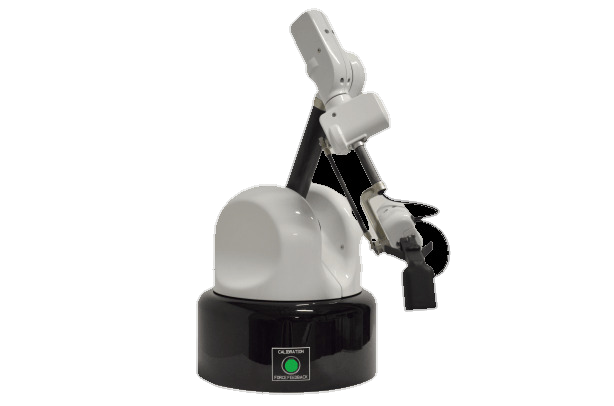
\includegraphics[width=22mm]{desktop-6D-compact-force-feedback-device-white.png}};
\node[font=\scriptsize, fill=white, inner sep=1pt, below=0.5mm of device] {Desktop 6D Compact};

% --- shared-autonomy hub: belief, policy, and arbitration nested in the group region ---
\node[sub, minimum width=18mm] (sabel) at (3.0,8.85) {Belief\\(goal probability)};
\node[sub, minimum width=18mm] (sapol) at (5.9,8.85) {Optimal\\policy};
\node[sub, minimum width=28mm] (saarb) at (4.45,7.55) {Arbitration};
\begin{pgfonlayer}{background}
\node[fit=(sabel)(sapol)(saarb), fill=orange!7, draw=orange!55!black,
      line width=0.7pt, rounded corners=4pt, inner sep=3.4mm] (sagrp) {};
\end{pgfonlayer}
\node[tagl, orange!55!black, anchor=south west] at ($(sagrp.north west)+(1mm,0.8mm)$) {shared autonomy};

% --- safety controller: reference governor, QP, and collision manager ---
\node[blk, minimum width=19mm] (gov) at (9.6,7.55) {Reference\\governor};
\node[blk, minimum width=23mm] (qp)  at (9.6,6.15) {CLF--CBF QP};
\node[blk, minimum width=21mm] (col) at (9.6,4.75) {Collision\\manager};
\begin{pgfonlayer}{background}
\node[fit=(gov)(qp)(col), fill=blue!6, draw=blue!45!black,
      line width=0.7pt, rounded corners=4pt, inner sep=3.4mm] (bluegrp) {};
\end{pgfonlayer}
\node[tagl, blue!45!black, anchor=south west] at ($(bluegrp.north west)+(1mm,0.8mm)$) {safety controller};

\node (robot) at (12.85,6.15) {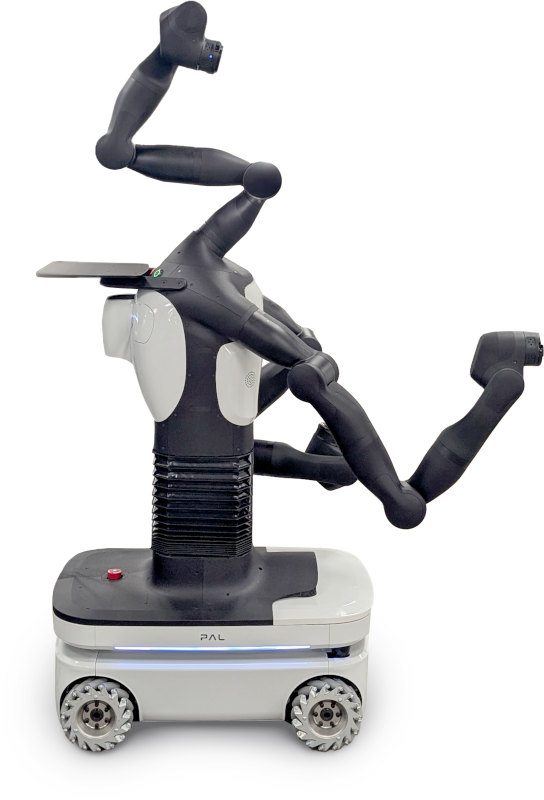
\includegraphics[width=20mm]{triago.png}};
\node[font=\scriptsize, fill=white, inner sep=1pt, below=0.5mm of robot] {TRIAGo};

% --- perception and world: dual world branch merges before the collision manager, kept close to the hub it feeds ---
\node[blk, minimum width=21mm] (yaml) at (4.5,2.85) {Static world\\(YAML)};
\node[blk, minimum width=21mm] (perc) at (7.9,2.85) {Perceived world\\(latched snapshot)};
\node[blk, minimum width=21mm] (head) at (7.9,1.55) {Head\\perception};
\begin{pgfonlayer}{background}
\node[fit=(yaml)(perc)(head), fill=black!4, draw=black!45,
      line width=0.7pt, rounded corners=4pt, inner sep=3.4mm] (greygrp) {};
\end{pgfonlayer}
\node[tagl, black!45, anchor=south west] at ($(greygrp.north west)+(1mm,0.8mm)$) {perception \& world};
\coordinate (wsel) at (6.2,3.8);

% --- always-on pipeline: operator to robot ---
\draw[bicore] (operator) -- (device);
\draw[core] (device.east) -- (1.1,7.85) -- node[above, fill=white, inner sep=1pt]{user twist $v_h$} ($(saarb.west)+(0,0.3)$);
\draw[core] (sabel.south) -- ($(saarb.north)+(-0.7,0)$);
\draw[core] (sapol.south) -- ($(saarb.north)+(0.7,0)$);
\draw[core] (gov) -- (qp);
\draw[core] (col) -- node[right, fill=white, inner sep=1pt]{$J_{\text{soft}},h_{\text{soft}}$} (qp);
\draw[core] (qp.east) -- node[above]{$\qdot^{\star}$} (robot.west);

% --- QP dual feedback to arbitration: straight edge, flat horizontal label ---
\draw[core] (qp.west) -- (8.2,6.15) -- (8.2,6.8) -- (5.35,6.8) -- ($(saarb.south)+(0.9,0)$);
\node[anchor=south, fill=white, inner sep=1pt] at (6.6,6.8) {$\lambda_{\text{cbf}}$};

% --- dual world sources merge at a junction: dashed in (alternative sources), solid out (one selected) ---
\draw[selArr, densely dashed] (yaml.south) -- (wsel);
\draw[selArr, densely dashed] (perc.south) -- (wsel);
\draw[selArr] (wsel) -- (col.south);
\draw[core] (head.north) -- node[right, font=\scriptsize\itshape]{camera} (perc.south);
\fill[black!55] (wsel) circle (0.5mm);
\draw[selArr] (wsel) -- (3.55,3.8) -- ($(saarb.south)+(-0.9,0)$);
\node[anchor=west, fill=white, inner sep=1pt, font=\scriptsize\itshape] at (3.65,5.5) {world};

% --- Channel B: outgoing reference is optionally blended just before the governor, always delivered ---
\draw[draw=black, line width=0.5pt] (saarb.east) -- node[above, pos=0.5, fill=white, inner sep=1pt]{reference} (8.1,7.55);
\draw[draw=black, line width=0.5pt, densely dashed] (8.1,7.55) -- (8.5,7.55);
\draw[core] (8.5,7.55) -- (gov.west);
\node[tagl, orange!85!black] at (8.4,7.9) {B};

% --- Channel F: guidance force closing the haptic loop, fully optional connection ---
\draw[optF] ($(saarb.west)+(0,-0.2)$) -- (-1.15,7.35) -- (-1.15,8.05) -- (-0.25,8.05);
\node[tagl, orange!85!black] at (1.9,7.0) {F};
\node[anchor=south, fill=white, inner sep=1pt] at (0.35,7.35) {$F_{\text{guide}}$};

\end{tikzpicture}
\caption{Ellipses denote human or physical endpoints, rounded rectangles denote software nodes, and a light tint groups and labels each cluster. A dashed segment marks a choice fixed by the study condition, namely the guidance force to the operator (channel F), whether the outgoing reference was blended before always reaching the governor (channel B), or the choice between the static and perceived world sources, of which exactly one is active. Channels F and B are independent, so either, both, or neither may be on.}
\label{fig:arch}
\end{figure}

%───────────────────────────────────────────────────────────────────────────────
\section{Task setting and world model}
\label{sec:task}

The robot works at a fixed tabletop workcell. Rigid cylinders of known radius stand on the table; each must be picked up, transported, and set upright on a delivery station --- a conveyor infeed or an intermediate handover disk --- mounted on a unit beside the table. A cylinder admits two grasp families: a \emph{top grasp}, approaching along world $-Z$ with a free roll about the cylinder axis, and a \emph{side grasp}, approaching horizontally at a free azimuth and a free height along the body. Which family is usable in a layout is fixed by the overhead clearance --- a shelf or canopy over the table closes the top corridor and forces side grasps, an unobstructed ceiling admits top grasps. A layout may also place a delivery station within reach of only one arm, so that clearing the table requires the arms to hand a cylinder between them, or it may give each arm a station within its own reach; the two cases exercise, respectively, the coordinated and the independent behaviour of the bimanual controller. The concrete layouts used for evaluation are specified in Section~\ref{sec:studyworld}.

Two representations of this scene coexist and are kept distinct. The \emph{visual} scene carries full industrial dressing --- fences, gantries, cabinets, the stations' own frames --- for the operator's spatial context only. The \emph{collision} world seen by the safety controller is a separate, deliberately small set of declared convex colliders: the table, each cylinder, the layout's blocking structure, and one convex envelope per station unit. The forward-invariance guarantees of Section~\ref{sec:cbf} and Section~\ref{sec:jl} are stated over this declared model, so a fixture that is drawn but not declared lies outside them by construction. A cylinder is a world obstacle until grasped; on grasp it is attached to the gripper frame and carried with the arm as a moving collider (Section~\ref{sec:grasp}).

The shared-autonomy layer represents every admissible grasp and every admissible placement as a goal (Section~\ref{sec:policies}). Figure~\ref{fig:goalposes} shows the resolved goal poses for a representative layout.

\begin{figure}[t]
\centering
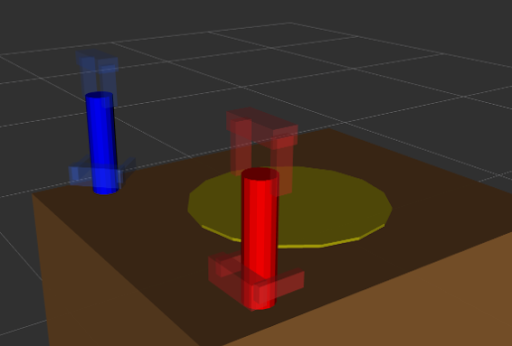
\includegraphics[width=0.75\linewidth]{goal-poses.png}
\caption{Resolved goal poses for a representative layout, shown in RViz. Each of the two cylinders carries a translucent gripper model at its resolved top-grasp pose (approach along world $-Z$) and at its resolved side-grasp pose (horizontal approach), both resolved against the current end-effector anchor (Section~\ref{sec:policies}); the yellow disk is a placement platform. The table and cylinders are the declared collision colliders.}
\label{fig:goalposes}
\end{figure}

%───────────────────────────────────────────────────────────────────────────────
\section{QP-CLF-CBF safety controller}
\label{sec:qp}

\subsection{Decision variables and complete formulation}

Let $n_v$ be the velocity dimension of the full kinematic model~\cite{carpentier2019} and let $\mathcal{A}$ denote the index set of the 14 actuated arm joints (7 per arm; every other joint --- head, torso, base, grippers --- is locked, see below). The decision vector is
\begin{equation}
x \;=\; \bigl[\,\qdot \in \mathbb{R}^{n_v},\;\; \delta_R,\;\; \delta_L\,\bigr] \in \mathbb{R}^{n_v+2},
\end{equation}
where $\qdot$ is the commanded joint velocity and $\delta_R,\delta_L$ are scalar tracking-relaxation (slack) variables, one per arm. Every control tick the following strictly convex QP --- a control Lyapunov function (CLF)--control barrier function (CBF) safety filter in the standard form of~\cite{ames2017cbf,ames2019ecc} --- is solved:
\begin{equation}
\label{eq:cost}
\min_{\qdot,\,\delta_R,\,\delta_L} \;\;
\underbrace{\sum_{i=1}^{n_v}\lambda_i\,\qdot_i^{\,2}}_{\text{damping}}
\;+\; \underbrace{w_c\!\!\sum_{i\in\mathcal{A}}\bigl(\qdot_i - v_i^{\text{post}}\bigr)^2}_{\text{posture field}}
\;+\; \underbrace{w_{\delta,R}\,\delta_R^2 + w_{\delta,L}\,\delta_L^2}_{\text{CLF slack}}
\;+\; \underbrace{\sum_{i\in\mathcal{A}} \rho_i\bigl(\qdot_i - \qdot_i^{\text{meas}}\bigr)^2}_{\text{rate damping}}
\end{equation}
subject to, for each arm $X \in \{R, L\}$:
\begin{align}
\hat{e}_{w,X}^{\top} J_{\text{task},X}\,\qdot \;+\; \delta_X \;&\ge\; \hat{e}_{w,X}^{\top}\dot{x}_{\text{ref},X} + \tfrac{\gamma_X}{2}\,\|e_{w,X}\| && \text{(CLF, Section~\ref{sec:clf})} \label{eq:clf}\\[2pt]
J_{\text{soft},X}\,\qdot \;&\ge\; -\gamma_{\text{cbf}}\,\bigl(h_{\text{soft},X} - d_{\text{safe},X}\bigr) && \text{(CBF, Section~\ref{sec:cbf})} \label{eq:cbf}\\[2pt]
\qdot_{\min,i}^{\text{safe}} \;\le\; \qdot_i \;&\le\; \qdot_{\max,i}^{\text{safe}} \qquad \forall i && \text{(joint limits, Section~\ref{sec:jl})} \label{eq:jl}
\end{align}
Here:
\begin{itemize}[nosep]
\item $\lambda_i$ is the $i$-th component of the per-joint damping weight vector, defined from a single scalar base damping $\lambda > 0$ as $\lambda_i = \lambda$ for every joint, raised on the joints of an arm that is currently \emph{frozen} (not teleoperated), which decouples its solution from the active arm's demands (Appendix~\ref{app:config}). (Throughout, bare $\lambda$ denotes this damping scalar; Lagrange multipliers are always subscripted, e.g.,\ $\lambda_{\text{cbf}}$, $\lambda_{\text{jl}}$ --- see Section~\ref{sec:sched});
\item $v^{\text{post}}$ is the posture-field reference velocity and $w_c$ its scalar weight (Section~\ref{sec:posture}), nonzero only on $\mathcal{A}$;
\item $w_{\delta,X}$ is the adaptively scheduled slack weight of arm $X$ (Section~\ref{sec:sched});
\item $\rho_i$ is the per-arm \emph{scheduled} rate-damping weight and $\qdot^{\text{meas}}$ the \emph{measured} joint velocity (Section~\ref{sec:rate}); the term exists only on $\mathcal{A}$;
\item $e_{w,X} = W_{\text{task}}\,e_X$ is the diagonally weighted task error of arm $X$, $\hat{e}_{w,X}$ its unit vector, $J_{\text{task},X}$ the arm's 6D frame Jacobian, $\dot{x}_{\text{ref},X}$ the reference feed-forward twist, and $\gamma_X$ the arm's CLF convergence rate;
\item $J_{\text{soft},X}$, $h_{\text{soft},X}$ are arm $X$'s SoftMin collision-barrier gradient and value, $d_{\text{safe},X}$ its velocity-dependent safety margin, $\gamma_{\text{cbf}}$ the class-$\mathcal{K}$ barrier gain.
\end{itemize}
Joints outside $\mathcal{A}$ are hard-locked to zero velocity by two opposing rows of~\eqref{eq:jl} ($0 \le \qdot_i \le 0$), rendering the head, torso, base, and grippers kinematically frozen from the QP's perspective. Every cost term leaves a zero gradient on those locked joints, a requirement for feasibility (Section~\ref{sec:rate}).

The QP is solved with a dual active-set method (Goldfarb--Idnani~\cite{goldfarb1983}, \texttt{quadprog}). On the rare infeasible tick the commanded velocity is zeroed for that tick (safe halt).

\subsection{CLF --- task tracking with relaxation}
\label{sec:clf}

For each arm, the task error is $e_X = x_{\text{ref},X} - x_X$ --- stacked position error and orientation error ($\log_3$ of the relative rotation). Let $W_{\text{task}}$ be the diagonal, strongly position-dominant task-weight matrix, $e_{w,X} = W_{\text{task}}\,e_X$ the weighted error, and $\hat{e}_{w,X} = e_{w,X}/\|e_{w,X}\|$ its unit direction (for $e_{w,X} \neq 0$); the position dominance of $W_{\text{task}}$ is what makes orientation yield first when tracking and safety conflict.

Row~\eqref{eq:clf} is the relaxed decrease condition for the \emph{weighted-error norm} as Lyapunov candidate. With $\dot{e}_X = \dot{x}_{\text{ref},X} - J_{\text{task},X}\,\qdot$,
\begin{equation}
V_X = \|e_{w,X}\|,
\qquad
\dot{V}_X = \hat{e}_{w,X}^{\top}\dot{e}_X
= \hat{e}_{w,X}^{\top}\dot{x}_{\text{ref},X} - \hat{e}_{w,X}^{\top} J_{\text{task},X}\,\qdot,
\label{eq:clfnorm}
\end{equation}
a positive-definite, radially unbounded candidate, continuously differentiable away from $e_{w,X} = 0$ --- admissible, if non-smooth at the origin (Section~\ref{sec:sota-clf-cbf-qp}). The task weighting enters \emph{once}, through the unit direction $\hat{e}_{w,X}$, which is then contracted with the plain frame Jacobian and feed-forward twist: this keeps the row a \emph{unit-gradient} constraint at every error magnitude, whereas carrying $W_{\text{task}}$ a second time through the rate would reinstate a $W_{\text{task}}^2$ scaling. Imposing the relaxed exponential decrease $\dot{V}_X \le -\tfrac{\gamma_X}{2}\,V_X + \delta_X$ with slack $\delta_X \ge 0$ and rearranging returns~\eqref{eq:clf} exactly. Positivity of $\delta_X$ is implicit --- it enters no other constraint and is quadratically penalised, so the optimum never drives it below what the row requires.

The classical alternative is the quadratic candidate $V_X^{q} = \tfrac{1}{2}\,e_X^{\top} W_{\text{task}}\,e_X$, whose decrease condition
\begin{equation}
(W_{\text{task}}e_X)^{\top} J_{\text{task},X}\,\qdot + \delta_X
\;\ge\;
(W_{\text{task}}e_X)^{\top}\dot{x}_{\text{ref},X} + \gamma_X\, V_X^{q}
\label{eq:clfquad}
\end{equation}
has a row vector $W_{\text{task}}e_X$ and a closing-speed demand $\gamma_X V_X^{q}$ that both scale \emph{quadratically} with $e_X$ --- near-singular rows far from the reference, vanishing tracking authority close to it. The normalised row~\eqref{eq:clf} keeps the same descent direction ($\hat{e}_{w,X}$ is the normalised gradient of $V_X^{q}$) but demands a decrease \emph{linear} in the error, so one row is well conditioned in free-space reaching and in millimetric terminal convergence alike.

The slack is the single most important design element for feasibility: because $\delta_X$ appears only in arm $X$'s CLF row and in the cost, the CLF can \emph{always} yield to the hard constraints \eqref{eq:cbf}--\eqref{eq:jl}. Tracking degrades gracefully under conflict; safety never does.

\subsection{CBF --- per-arm SoftMin collision barrier}
\label{sec:cbf}

Collision avoidance is enforced over a capsule-based geometric model of both arms (dominant-axis-snapped capsules per link, box-approximated grippers, body/ground/wall colliders). The declared pairs cover each arm against the world obstacles, each arm against the other, each arm against itself (its distal hand against its own proximal links), and each arm against the head chain, whose live forward-kinematic capsules enter as a quasi-static obstacle with no head joint in the QP decision vector. Each tick, all declared pairs are queried for signed distance $d_k(q)$; pairs within a filter radius are sorted and the $K$ closest retained.

A single minimum-distance constraint is non-smooth, so the barrier aggregates the active set through a SoftMin --- a log-sum-exp composition in the spirit of nonsmooth barrier composition~\cite{glotfelter2017}. The key architectural decision is a \emph{per-arm decomposition}: two independent barriers are assembled, where $\mathcal{P}(X)$ is the subset of active pairs touching at least one geometry belonging to arm $X$ (its own links and gripper, or a cylinder it currently holds):
\begin{align}
h_{\text{soft},X}(q) &= -\frac{1}{\alpha_s}\,\log\!\!\sum_{k \in \mathcal{P}(X)} e^{-\alpha_s d_k(q)},
&
J_{\text{soft},X}(q) &= \sum_{k \in \mathcal{P}(X)} \sigma_k\, J_k(q),
\quad
\sigma_k = \frac{e^{-\alpha_s d_k}}{\sum_{j \in \mathcal{P}(X)} e^{-\alpha_s d_j}},
\label{eq:softmin}
\end{align}
where $\alpha_s$ is the aggregation sharpness, $J_k$ is pair $k$'s distance Jacobian (witness-point Jacobian difference projected on the witness normal), and $\sigma_k$ are softmax weights. $h_{\text{soft},X}$ is a smooth lower approximation of the true minimum distance restricted to arm $X$'s pairs, and $J_{\text{soft},X}$ is the convex blend of exactly those pairs' Jacobians --- hence it has zero columns in the \emph{other} arm's joints unless a pair genuinely involves both arms. A genuine inter-arm pair contributes to both $\mathcal{P}(R)$ and $\mathcal{P}(L)$, preserving the ability of either arm to yield for the other.

Without the split, a single SoftMin row would mix all pairs and let the QP recruit the idle arm's joints to cheaply satisfy a barrier activated solely by the active arm near an unrelated obstacle, producing spurious idle-arm motion and oscillation. The same coupling concern applies to the safety margin, which is therefore also split per arm:
\begin{equation}
d_{\text{safe},X} \;=\; d_0 + k_v\,\|\qdot_X\|,
\label{eq:dsafe}
\end{equation}
computed from each arm's \emph{own} joint-velocity norm $\|\qdot_X\|$ (base margin $d_0$, velocity horizon $k_v$).

Constraint~\eqref{eq:cbf} then enforces the class-$\mathcal{K}$ barrier condition $\dot{h} \ge -\gamma_{\text{cbf}}\,(h - d_{\text{safe}})$ on each arm's aggregate: the arm may approach an obstacle only at a rate that vanishes as the margin approaches $d_{\text{safe},X}$, rendering the safe set forward-invariant (up to the SoftMin approximation error, which is conservative).

The aggregation sharpness $\alpha_s$ is set to a high value, for a reason that becomes acute in cluttered geometry. The log-sum-exp in~\eqref{eq:softmin} under-approximates the true minimum distance over $\mathcal{P}(X)$ by at most $\alpha_s^{-1}\ln|\mathcal{P}(X)|$, so a larger $\alpha_s$ both tightens $h_{\text{soft},X}$ onto $\min_k d_k$ and concentrates the softmax weights $\sigma_k$ onto the genuinely nearest pair. When an arm is boxed in --- a table below, a shelf above, structural legs alongside --- many pairs sit at nearly equal distance while their witness normals point in genuinely different directions. A low $\alpha_s$ then averages those directions in $J_{\text{soft},X}$ toward mutual cancellation, shrinking $\|J_{\text{soft},X}\|$ with no real loss of clearance; through~\eqref{eq:cbf} this drives up the collision shadow price $\lambda_{\text{cbf},X}$ (Section~\ref{sec:sched}) --- which varies roughly as $\|J_{\text{soft},X}\|^{-2}$ --- and inflates the apparent cost of a clearance deficit that is not physically present. A sharp $\alpha_s$ keeps the blend~\eqref{eq:softmin} dominated by the single closest pair, so $J_{\text{soft},X}$ retains the magnitude and direction of a true nearest-obstacle gradient.

\subsection{Posture task --- gradient potential field}
\label{sec:posture}

Redundancy not consumed by the tracking row is shaped by a posture field: the negative gradient of a scalar joint-limit potential, folded into the QP cost~\eqref{eq:cost} rather than projected through the null space, so the solver arbitrates it against tracking and the hard rows instead of subordinating it to them. The potential is an inverse-square repulsive barrier --- the joint-limit counterpart of the gradient-projection criteria of Li\'egeois~\cite{liegeois1977} and of Zghal, Dubey, and Euler~\cite{zghal1990} --- with one term per bound and the distance-to-limit in place of a distance-to-obstacle. It is evaluated on the \emph{normalised} joint coordinate, so every joint is defended at the same fraction of its travel toward whichever bound it approaches. For joint $i$ with limits $[q_i^{\ell}, q_i^{u}]$, midpoint $\bar{q}_i$, and half-range $\Delta_i = \tfrac{1}{2}(q_i^{u} - q_i^{\ell})$:
\begin{align}
p_i &= \operatorname{clip}\!\Bigl(\frac{q_i - \bar{q}_i}{\Delta_i},\, -1+\varepsilon,\, 1-\varepsilon\Bigr),
&
H(p) &= \frac{1}{(1-p)^2} + \frac{1}{(1+p)^2},
\\
\frac{dH}{dp} &= \frac{2}{(1-p)^3} - \frac{2}{(1+p)^3},
&
v_i^{\text{post}} &= \operatorname{clip}\!\Bigl(-k_g\,\frac{dH}{dp}\Big|_{p_i},\; \pm v_{\max}^{\text{post}}\Bigr),
\end{align}
where $k_g$ is the gradient gain, $v_{\max}^{\text{post}}$ a hard clamp for solver safety, and the interior clamp $\varepsilon$ keeps the gradient finite and correctly signed even at or beyond a limit --- the raw cube would flip sign there and drive the joint \emph{out}. At the midpoint $p_i = 0$, so $dH/dp = 0$ and $v_i^{\text{post}}$ vanishes; toward either bound $|p_i| \to 1$ and $H$ diverges. The field is therefore negligible through mid-range --- leaving full redundancy to the CLF --- and grows sharply only near a limit. During autonomous precision phases the posture weight $w_c$ is smoothly ramped to a small fraction of its nominal value by a first-order filter, so the QP spends the redundancy on tracking rather than centring.

\subsection{Rate damping --- measured-velocity anchor}
\label{sec:rate}

The rate term in~\eqref{eq:cost} penalises deviation from the \emph{measured} joint velocity $\qdot^{\text{meas}}$ on the active joints $\mathcal{A}$. Under a position-dominant $W_{\text{task}}$ the wrist directions are task-null for~\eqref{eq:clf} and are resolved by the cost alone, which without this term carries no memory of the previous tick; the anchor supplies that memory from the arm's physical state. Two properties are structural. The anchor is the measured velocity and not the controller's own previous output $\qdot^{\star}_{k-1}$, which would insert a self-referential low-pass filter into the forward path of the closed loop and pull the command toward the controller's internal history rather than the arm's state. The restriction to $\mathcal{A}$ is a feasibility requirement: joints outside $\mathcal{A}$ are already pinned by two opposing rows of~\eqref{eq:jl}, and $\qdot^{\text{meas}}$ carries motion and differentiation noise on exactly those joints, so an unmasked term would contest the pin and force two linearly dependent rows into the active set at once. The weight $\rho_i$ trades tracking against damping and is scheduled per arm between two values (Appendix~\ref{app:config}), full only near convergence: at large error a strong pull toward a near-zero measured velocity re-suppresses every departing command and stalls the arm.

\subsection{Adaptive scheduling via KKT shadow prices}
\label{sec:sched}

The QP's dual solution is exploited as a feedback signal. After each solve, the Karush--Kuhn--Tucker (KKT) Lagrange multipliers of the two CBF rows ($\lambda_{\text{cbf},R},\lambda_{\text{cbf},L}$) and of the joint-limit rows ($\lambda_{\text{jl}}$, reduced to a per-arm maximum) are extracted --- these \emph{shadow prices} measure exactly how much the optimal cost would improve per unit relaxation of the corresponding constraint~\cite{boyd2004}, i.e.,\ how hard each safety constraint is actively fighting the task. Raw multipliers are noisy tick-to-tick (active-set changes are discrete events), so each multiplier $\lambda_{(\cdot)}$ is smoothed by a first-order low-pass with time constant $\tau_{\lambda}$:
\begin{equation}
\bar{\lambda}_{(\cdot)} \leftarrow \kappa\,\bar{\lambda}_{(\cdot)} + (1-\kappa)\,\lambda_{(\cdot)}, \qquad \kappa = e^{-\Delta t/\tau_{\lambda}}.
\end{equation}
The slack weight $w_{\delta,X}$ is scheduled \emph{per arm} from the driver $\bar{\lambda}_X = \max\bigl(\bar{\lambda}_{\text{cbf},X},\, \bar{\lambda}_{\text{jl},X}\bigr)$ --- that arm's own collision shadow price or its own joint-limit shadow price, whichever is larger --- through a quadratic-tolerance law. That law alone is not sufficient: even a smoothly-varying $\bar\lambda_X$ can cross the map's steep knee and produce a large one-tick jump in the weight, since the map's local sensitivity $\beta$ is unbounded near that knee. The schedule therefore filters its own \emph{output}, not only the input $\bar\lambda_X$, as a second independent LPF stage:
\begin{equation}
w_{\delta,X}^{\text{tgt}} \;=\; w_{\delta}^{\text{base}} + e^{-\beta\,\bar{\lambda}_X^2}\,\bigl(w_{\delta}^{\max} - w_{\delta}^{\text{base}}\bigr),
\qquad w_{\delta,X} \leftarrow \text{LPF}_{\tau_{w}}\bigl(w_{\delta,X}^{\text{tgt}}\bigr),
\label{eq:slacksched}
\end{equation}
each arm carrying its own persistent LPF state. In free space ($\bar{\lambda}_X\to 0$) arm $X$'s slack weight rises to its ceiling $w_{\delta}^{\max}$ (tight tracking, expensive to relax); near an active constraint on that arm it drops toward its base $w_{\delta}^{\text{base}}$ (tracking yields cheaply, preserving safety authority) --- independently of the other arm. A frozen arm bypasses the schedule, its slack weight pinned at the ceiling so the hold is rigid; an arm executing an autonomous grasp is pinned identically so that alignment converges inside tolerance.

\subsection{Joint limits --- per-joint position-limit barrier}
\label{sec:jl}

Each actuated joint must stay inside its mechanical range, so the set to render forward-invariant is the joint-space box
\begin{equation}
\mathcal{C}_q \;=\; \bigl\{\, q \;:\; q_i^{\ell} \le q_i \le q_i^{u}\ \ \forall i \,\bigr\},
\label{eq:jlset}
\end{equation}
the intersection of the per-joint slabs $\mathcal{C}_i = \{\,q : q_i^{\ell} \le q_i \le q_i^{u}\,\}$. The arms are commanded at the velocity level, so each joint is a single integrator $\dot{q}_i = \qdot_i$ with $\qdot_i$ a decision variable, and forward invariance of $\mathcal{C}_q$ is secured by one linear barrier per bound. Let $d_i^{+} = q_i^{u} - q_i$ and $d_i^{-} = q_i - q_i^{\ell}$ be the distances to the upper and lower limit; each is $C^1$ and positive on the interior of its slab. With a speed-dependent buffer $b_i = b_0 + k_b\,\lvert\qdot_i^{\text{meas}}\rvert$ --- base margin $b_0 > 0$ and horizon gain $k_b > 0$ acting on the measured joint speed $\lvert\qdot_i^{\text{meas}}\rvert$ --- the barrier guarding the upper bound is $h_i^{+} = d_i^{+} - b_i$ and the one guarding the lower bound is $h_i^{-} = d_i^{-} - b_i$, each positive while the joint sits more than $b_i$ from that limit. Imposing the class-$\mathcal{K}$ barrier condition $\dot{h}_i^{+} \ge -k_p\,h_i^{+}$ with linear gain $k_p > 0$ and substituting the single-integrator kinematics $\dot{d}_i^{+} = -\qdot_i$, with $b_i$ held constant over one tick so that $\dot{h}_i^{+} \approx \dot{d}_i^{+}$, reduces the condition to a plain upper bound on the joint velocity, $\qdot_i \le k_p\,(d_i^{+} - b_i)$. The lower bound follows the same way from $h_i^{-}$, where $\dot{d}_i^{-} = \qdot_i$ gives $\qdot_i \ge -k_p\,(d_i^{-} - b_i)$. Combined with the model's hard velocity limit $\bar{v}_i$, these are the box~\eqref{eq:jl} bounds
\begin{equation}
\qdot_{\max,i}^{\text{safe}} = \min\!\bigl(\bar{v}_i,\; k_p(d_i^{+} - b_i)\bigr),
\qquad
\qdot_{\min,i}^{\text{safe}} = -\min\!\bigl(\bar{v}_i,\; k_p(d_i^{-} - b_i)\bigr).
\label{eq:jlbrake}
\end{equation}
Invariance follows from Nagumo's theorem~\cite{blanchini1999,ames2019ecc}: on the face $q_i = q_i^{u}$ the admissible interval collapses to $\qdot_i \le -k_p b_i < 0$, so any $\qdot$ satisfying the row points strictly into $\mathcal{C}_q$, and likewise on the lower face. The barrier is linear and one per bound, so the joint limits enter the QP as a hard box with no aggregation and no relaxation, unlike the collision barrier of Section~\ref{sec:cbf}. The buffer keeps the trajectory a margin $b_i$ inside the mechanical stop, and its growth with $\lvert\qdot_i^{\text{meas}}\rvert$ offsets the one-tick sampling lag, so the inward-pointing property survives discretisation and a fast joint begins braking earlier.

\subsection{Reference governor}
\label{sec:governor}

An intermediate layer between the raw Cartesian reference and the CLF --- a reference-governor scheme~\cite{garone2017} --- guarantees that the reference the CLF perceives always lives in a constraint-admissible set, preserving QP feasibility under discontinuous, aggressive, or far-away commands without modifying the QP itself (Algorithm~\ref{alg:governor}). The governor is transparent when the reference is well-behaved (output $\equiv$ input), stateful per arm (velocity memory $v^{\text{prev}}$ for the acceleration clamp, reset on arm switch or watchdog freeze), and adds no rows to the QP.

\begin{algorithm}[t]
\caption{Reference governor (one arm, one control tick).}
\label{alg:governor}
\small
\KwIn{raw reference $(x_{\text{ref}}, R_{\text{des}}, v_{\text{ref}}, \omega_{\text{ref}})$; real EE pose $(x, R)$; previous governed velocities $(v^{\text{prev}}, \omega^{\text{prev}})$; timestep $\Delta t$}
\KwOut{governed reference $(x_g, R_g, v_g, \omega_g)$ passed to the CLF}
\tcc{1. Velocity shaping (magnitude clamp, direction preserved)}
$v_g \leftarrow v_{\text{ref}}\cdot\min\bigl(1,\, V_{\max}^{\text{lin}}/\|v_{\text{ref}}\|\bigr)$\;
$\omega_g \leftarrow \omega_{\text{ref}}\cdot\min\bigl(1,\, V_{\max}^{\text{ang}}/\|\omega_{\text{ref}}\|\bigr)$\;
\tcc{2. Position-error bounding (project onto the admissible ball)}
\eIf{$\|x_{\text{ref}} - x\| > E_{\max}^{\text{pos}}$}{
  $x_g \leftarrow x + E_{\max}^{\text{pos}}\,\dfrac{x_{\text{ref}} - x}{\|x_{\text{ref}} - x\|}$\;
}{
  $x_g \leftarrow x_{\text{ref}}$\;
}
\tcc{3. Acceleration limiting (rate-limit $\Delta v$, then re-clamp magnitude)}
$\Delta v \leftarrow v_g - v^{\text{prev}}$\;
$v_g \leftarrow v^{\text{prev}} + \Delta v \cdot \min\bigl(1,\, A_{\max}^{\text{lin}}\Delta t/\|\Delta v\|\bigr)$\;
$\Delta \omega \leftarrow \omega_g - \omega^{\text{prev}}$\;
$\omega_g \leftarrow \omega^{\text{prev}} + \Delta \omega \cdot \min\bigl(1,\, A_{\max}^{\text{ang}}\Delta t/\|\Delta \omega\|\bigr)$\;
re-apply step 1 to $(v_g, \omega_g)$\;
$v^{\text{prev}} \leftarrow v_g$;\quad $\omega^{\text{prev}} \leftarrow \omega_g$\;
\tcc{4. Orientation geodesic clamping (bounded angular demand, avoids the $\pi$ singularity)}
$R_{\text{err}} \leftarrow R_{\text{des}}R^{\top}$;\quad $\theta \leftarrow \|\log_3 R_{\text{err}}\|$\;
\eIf{$\theta > E_{\max}^{\text{ori}}$}{
  $R_g \leftarrow \exp_3\!\Bigl(\dfrac{E_{\max}^{\text{ori}}}{\theta}\log_3 R_{\text{err}}\Bigr)R$\;
}{
  $R_g \leftarrow R_{\text{des}}$\;
}
\end{algorithm}

%───────────────────────────────────────────────────────────────────────────────
\section{Filtered quantities and the delay they introduce}
\label{sec:filtering}

Several quantities in this architecture are low-pass filtered before use: the shadow prices and the slack weight they drive~\eqref{eq:slacksched}, the autonomy authority~\eqref{eq:alpha}, the guidance gain (Section~\ref{sec:guidance}), the resolved goal directions (Section~\ref{sec:policies}), and the posture-weight scale (Section~\ref{sec:posture}). Every filter is a delay, and a delay inside a control loop is a liability rather than free smoothing. This section states where filtering is admitted, what its delay costs, and why that cost is never paid on the safety guarantee.

\textbf{No filter lies between a measurement and a constraint.} The barrier value and its gradient~\eqref{eq:softmin}, the dynamic margin~\eqref{eq:dsafe}, the joint-limit bounds~\eqref{eq:jlbrake}, and the configuration all of them are evaluated at enter the QP on the tick they are computed. The constraint rows~\eqref{eq:clf}--\eqref{eq:jl} --- the only objects the forward-invariance arguments of Section~\ref{sec:cbf} and Section~\ref{sec:jl} rest on --- therefore see the present state and never a lagged one, so no amount of filtering elsewhere can postpone the controller's reaction to an approaching obstacle by a single tick. For the same reason the operator's command path carries a slew-rate limiter rather than a low-pass filter (Section~\ref{sec:device}): a rate limiter is exactly transparent, with zero phase lag, to every signal slower than its bound, whereas a low-pass filter lags all of them.

\textbf{What is filtered is a price, not a constraint.} Every filtered quantity is a cost weight, an authority scalar, or a reference direction. A first-order filter of time constant $\tau$ contributes a phase lag that, for signal content well below $\tau^{-1}$, is approximately a pure delay of $\tau$ seconds. Because these quantities appear only in the QP's objective, a lagged value displaces the optimum \emph{within} the feasible set: it can leave the solution momentarily mistuned, but it cannot make an infeasible point feasible and it cannot move a barrier row. A slack weight that is a fraction of a second stale prices the tracking row slightly wrong for that fraction of a second, while the set of admissible joint velocities is identical either way. The delay is spent on optimality, which is the quantity this architecture is willing to spend.

\textbf{One filter closes a loop through the robot, and it is there because the loop needs it.} The slack-weight schedule of Section~\ref{sec:sched} is genuine feedback: the multiplier is read from the solve, filtered, mapped to a weight, and returned to the next solve. Its sign is stabilising --- raising $w_{\delta,X}$ makes tracking relaxation expensive, so the QP yields less on the task and presses harder against the barrier, which raises $\bar\lambda_X$, which the schedule maps back to a \emph{lower} weight --- so the loop is negative. Negative feedback with lag is not automatically stable: it oscillates once the loop gain at the frequency of accumulated phase crossover exceeds unity, and the local sensitivity of the quadratic-tolerance map in~\eqref{eq:slacksched} is unbounded near its knee, so that gain is not small. The output-stage filter in~\eqref{eq:slacksched} is what bounds it: by limiting how fast the weight may move, it attenuates the loop exactly at the frequencies where the phase lag would otherwise sustain an oscillation. It is therefore not a smoother laid over a delay problem but the element that makes the loop stable, and its lag is the price of that stability rather than an unwanted side effect. The failure mode is bounded in any case --- because the loop reaches only a cost weight, its worst outcome is a slow variation in how stiffly the task is tracked near an obstacle, never a violated barrier, since the rows carrying the guarantee are the rows the loop cannot touch.

\textbf{Elsewhere the loop closes only through the operator, and the release path is unfiltered.} The authority, the guidance gain, and the resolved goal directions are computed from operator and belief signals, and the robot's response to them returns only by way of the operator, whose own corrective bandwidth lies far below the rate at which these quantities are recomputed; their filters contribute lag without closing a loop inside the machine. Where that lag would matter --- returning authority to an operator who has begun to disagree --- it is bypassed rather than tolerated: the suspensions of Section~\ref{sec:blend} force the authority to zero \emph{and} reset the filter state, so an override takes effect on the tick it is detected and is not delayed by the filter that smooths authority on the way up. Filtering is admitted on the path that grants assistance and excluded from the path that withdraws it.

The exponential forgetting in the belief recursion~\eqref{eq:beliefupdate} is not a filter in this sense. It is the discount of a recursive Bayesian estimator --- a modelling statement that older evidence of an operator's intention is less relevant than newer evidence --- and its time constant is a property of the intent model rather than a concession to measurement noise. Every filter time constant in the system is listed in Appendix~\ref{app:config}.

%───────────────────────────────────────────────────────────────────────────────
\section{Bimanual architecture and coupling guarantees}

Each arm has its own CLF row, CBF row, slack variable, and adaptive weight schedule. An arm not currently teleoperated is CLF-held at its last end-effector (EE) pose (zero-velocity reference) with pinned maximal slack weight, raised convergence rate, and raised damping --- ensuring it holds position rigidly yet can still yield if required by a genuinely shared inter-arm barrier. The QP always publishes solved velocities for \emph{both} arms, so that collision-avoidance motion is never discarded.

The head chain is modelled as a quasi-static CBF obstacle: its capsules are updated from live forward kinematics every tick, but its joints are velocity-locked to zero in the QP. The forward-invariance guarantee degrades from exact to quasi-static-valid, bounded by the head's own displacement per control tick, $\|v_{\text{head}}\|/f_{\text{ctrl}}$ --- orders of magnitude below the base safety margin $d_0$ at the control rate $f_{\text{ctrl}}$ (Appendix~\ref{app:config}). This half alone is not sufficient: the dynamic margin~\eqref{eq:dsafe} thickens with the arm's \emph{own} joint-velocity norm only, so a moving head acts on this barrier as an unmodelled disturbance; the symmetric half --- a barrier on the head chain whose margin does see the head's own speed --- is imposed on the head-controller side (Section~\ref{sec:headtrack}).

%───────────────────────────────────────────────────────────────────────────────
\section{Shared autonomy}
\label{sec:sa}

Each tick the shared-autonomy layer (i)~computes one optimal policy per goal, (ii)~updates a Bayesian belief over the goal set from the operator's twist, (iii)~arbitrates authority between the operator and the highest-belief policy, and (iv)~drives a grasp state machine; under blending it is the sole writer of the arm reference.

\subsection{Goal set and goal manifolds}
\label{sec:policies}

For the task of Section~\ref{sec:task}, the goal set $\mathcal{G} = \{g_1,\dots,g_n\}$ contains, per graspable cylinder, a top-grasp and a side-grasp goal, plus one placement goal per placement platform the world declares (active only while holding an object); Figure~\ref{fig:goalposes} shows a resolved instance. We denote by $\mathcal{G}_{\text{act}} \subseteq \mathcal{G}$ the \emph{active} subset of goals that are currently demandable (Section~\ref{sec:belief}); all sums and maximisations below range over $\mathcal{G}_{\text{act}}$.

A cylinder does not prescribe one grasp pose: a side grasp is reached from any approach azimuth and at any height along the body, and a top grasp lifts the cylinder identically at any roll about its axis. Freezing these free directions into a single target would make the assistance fight the operator over choices the task does not care about. Each goal is therefore \emph{resolved} every tick, against an anchor pose, into the nearest task-equivalent target. The resolution anchor is the \emph{real} end-effector pose: it is always physically valid and slow-moving, whereas the operator's reference can momentarily fly through obstacles and would drag every goal manifold along with it. A world may declare several placement platforms; each becomes demandable by either arm once that arm holds a cylinder, and belief and guidance select which platform is active. A placement goal is resolved the same way: its only hard requirement is that the grasped cylinder's symmetry axis --- captured in the gripper frame at the instant of attachment --- end up vertical, a 2-DOF tilt constraint; the anchor position projected onto the platform, clamped inside its rim, chooses \emph{where} to place, the current gripper yaw about the vertical is preserved, and the demanded tilt is the minimal rotation onto the \emph{nearer} vertical, so the held object is never flipped end over end.

Each grasp resolves its free directions against the anchor. The top-grasp roll is obtained in closed form as the roll closest to the anchor orientation, with no candidates and no hysteresis. The side-grasp azimuth is a confidence-weighted blend of two estimates whose degeneracies do not coincide, so one is always well posed; its height is the anchor height clamped to the cylinder body. The one discrete choice, between the two finger orientations $180^{\circ}$ apart, is held by a distance-scaled hysteresis. Every resolved direction then passes through a normalised moving-average filter that bounds how fast a goal can travel around its manifold, so a degeneracy cannot slew the goal, and with it the guidance force.

\subsection{Local safe optimal policy}
\label{sec:localpolicy}

Every layer above the safety controller consumes the same primitive: for each active goal, the best motion toward that goal that is admissible \emph{here}, at the pose the arm currently occupies and under the obstacles currently near it. The belief compares this twist against the operator's, the arbitration blends it into the reference, and the haptic layer renders it as a force. It is built in two stages --- an attractive field that knows the goal and nothing else, and a projection that filters the field through the live safety constraint.

\textbf{Attractive field.} For a goal pose $T_g = (p_g, R_g)$ and current pose $T = (p, R)$, the field is a smoothly saturated proportional law,
\begin{align}
v_{\text{lin}} &= \frac{e}{\|e\|}\; v_{\max}\tanh\!\Bigl(\frac{K_p\,\|e\|}{v_{\max}}\Bigr),
&
\omega &= \frac{e_R}{\|e_R\|}\; \omega_{\max}\tanh\!\Bigl(\frac{K_p\,\|e_R\|}{\omega_{\max}}\Bigr),
\label{eq:vgeo}
\end{align}
where $e = p_g - p$ is the position error, $e_R = \log_3(R_g R^{\top})$ the axis--angle orientation error (with a guarded fallback near the $\pi$ singularity), $K_p > 0$ the proportional gain, and $v_{\max}, \omega_{\max} > 0$ the saturation speeds. Writing $v_{\text{geo},k} = (v_{\text{lin}}, \omega) \in \mathbb{R}^6$ for the stacked twist toward goal $g_k$, the linear channel is exactly the negative gradient of a scalar attractive potential,
\begin{equation}
U(e) \;=\; \frac{v_{\max}^{2}}{K_p}\,\ln\cosh\!\Bigl(\frac{K_p\,\|e\|}{v_{\max}}\Bigr),
\qquad
v_{\text{lin}} \;=\; -\nabla_{p}\,U(p_g - p),
\label{eq:attpot}
\end{equation}
and the angular channel is the same construction on the geodesic orientation error. $U$ is smooth, radially symmetric, and positive definite about the goal, with $U(e) \to \tfrac{1}{2}K_p\|e\|^{2}$ as $\|e\| \to 0$ and $U(e) \to v_{\max}\|e\|$ as $\|e\| \to \infty$: a spring of stiffness $K_p$ near the goal, a cone of constant slope $v_{\max}$ far from it. Linearity at the origin means the field vanishes smoothly \emph{at} the goal, so a guidance force rendered from it (Section~\ref{sec:guidance}) decays to zero instead of buzzing around a deadband edge; far-field saturation means the belief's evidence (Section~\ref{sec:belief}) compares twist \emph{directions} rather than distances, since a goal twice as far does not demand a twist twice as large. This is the attractive half of the classical potential-field construction~\cite{khatib1986}; what replaces its repulsive half is the next stage.

\textbf{Safety filter.} The field is blind to obstacles. The safety controller has already assembled, for the arm carrying the goal, that arm's aggregate barrier~\eqref{eq:softmin}, and publishes it in end-effector coordinates as a single row,
\begin{equation}
J_{\text{safe}} \;=\; J_{\text{soft},X}\,J_{\text{EE},X}^{+} \;\in\; \mathbb{R}^{1\times 6},
\qquad
b_{\text{safe}} \;=\; -\gamma_{\text{cbf}}\bigl(h_{\text{soft},X} - d_{\text{safe},X}\bigr) \;\in\; \mathbb{R},
\label{eq:jsafe}
\end{equation}
with $J_{\text{EE},X}^{+}$ the Moore--Penrose pseudoinverse of arm $X$'s end-effector Jacobian, so that a task twist $v$ advances the barrier of~\eqref{eq:cbf} at rate $J_{\text{safe}}\,v$ and counts as admissible here when $J_{\text{safe}}\,v \ge b_{\text{safe}}$. The pair $(J_{\text{safe}}, b_{\text{safe}})$ is the entire obstacle information available to this layer: a single half-space in twist space, recomputed each tick from the arm's real configuration.

The policy for goal $g_k$ is the admissible twist closest to the field in the task metric $W \succ 0$,
\begin{equation}
\pi_k \;=\; \arg\min_{v \in \mathbb{R}^6}\; \tfrac{1}{2}\,(v - v_{\text{geo},k})^{\top} W (v - v_{\text{geo},k})
\quad \text{s.t.} \quad J_{\text{safe}}\, v \ge b_{\text{safe}}.
\label{eq:policyqp}
\end{equation}
The feasible set is a closed half-space and the objective is strictly convex, so~\eqref{eq:policyqp} is a $W$-metric projection with a unique solution, and that solution is available in closed form. Stationarity of the Lagrangian of~\eqref{eq:policyqp} reads $W(\pi_k - v_{\text{geo},k}) = \mu\,J_{\text{safe}}^{\top}$ with multiplier $\mu \ge 0$, so the correction is confined to the single direction $W^{-1}J_{\text{safe}}^{\top}$; complementary slackness then leaves two cases, the constraint inactive with $\mu = 0$ and $\pi_k = v_{\text{geo},k}$, or the constraint active with $J_{\text{safe}}\,\pi_k = b_{\text{safe}}$, which determines $\mu$. Eliminating $\mu$ merges the two cases into
\begin{equation}
\pi_k \;=\; v_{\text{geo},k} \;+\; \frac{\bigl[\,b_{\text{safe}} - J_{\text{safe}}\,v_{\text{geo},k}\,\bigr]_{+}}{J_{\text{safe}}\,W^{-1}J_{\text{safe}}^{\top}}\;W^{-1}J_{\text{safe}}^{\top},
\label{eq:policyproj}
\end{equation}
with $[\,\cdot\,]_{+} = \max(\cdot,\,0)$. When the field already respects the barrier the policy \emph{is} the field, untouched. When it does not, the field is corrected by the smallest admissible increment, taken along the single direction $W^{-1}J_{\text{safe}}^{\top}$ --- the barrier gradient pulled through the inverse task metric --- and scaled exactly to bring the barrier to equality. Every component of the field with $J_{\text{safe}}\,v = 0$ is left intact, so the motion tangent to the obstacle survives the projection and the policy slides along the barrier instead of stopping in front of it. If the row is momentarily unavailable or inconsistent, the policy is a zero twist (a safe halt) --- never the unfiltered $v_{\text{geo},k}$, which could drive through the barrier.

Filtering through the safety layer's own live barrier, rather than through a private obstacle model, serves the estimator as much as the robot. Near an obstacle the operator's twist detours around the barrier, and against \emph{unfiltered} policies that detour would read as disagreement with every goal, corrupting the belief exactly where assistance matters most. Projected through the same barrier, all policies detour the same way, so the \emph{relative} costs in~\eqref{eq:cost-belief} keep discriminating between goals. Using the belief cost's own metric $W$ in~\eqref{eq:policyqp} closes the loop between inference and control: each $\pi_k$ is the admissible twist of maximal likelihood under its goal's observation model (Section~\ref{sec:belief}).

Two policy families are evaluated from the same goal resolution: \emph{robot policies}, anchored at the real end-effector (used for autonomous execution and belief-free guidance display), and \emph{user policies}, anchored at the pose the operator is actually steering --- the integrated clutch reference, the live end-effector in joystick mode (Section~\ref{sec:joystick}), or the blended reference when blending is active, i.e.,\ always the gripper the operator is watching --- with lower, teleoperation-comfortable saturation speeds. The user family feeds belief inference and haptic guidance, so the observation model is matched to achievable hand motion and the guidance field never demands speeds the hand cannot track. Both families aim at the same manifold point: the goal resolution, and its sticky-choice memory, is computed once at the end-effector anchor and shared.

\subsection{Locality of the policy and the role of the operator}
\label{sec:locality}

Equations~\eqref{eq:policyqp} and~\eqref{eq:policyproj} deliver, at every pose and for every goal, a twist that is safe by construction and optimal in the only sense this layer can evaluate --- the admissible motion closest to the steepest descent of that goal's potential. Read at face value, the robot can already solve the task by itself, and it is fair to ask what the operator is for. The answer is contained in the word \emph{local}, and it is structural rather than a matter of tuning.

The policy is a \emph{memoryless static feedback}. It is a function of the current pose, the current goal, and the barrier row evaluated at the current configuration from the currently nearest obstacle pairs; it holds no trajectory, no lookahead, and no representation of the free space beyond that one half-space. Under a single fixed goal the closed loop is therefore the autonomous system $\dot{T} = \pi_k(T)$. That structure is what buys real-time tractability and a hard safety certificate, and it fixes precisely what the policy cannot do. Three consequences follow.

\textbf{Equilibria away from the goal.} By~\eqref{eq:policyproj}, $\pi_k(T) = 0$ at a pose $T \neq T_{g_k}$ exactly when the barrier is active and the attractive field is cancelled by its own safety correction, that is, when
\begin{equation}
v_{\text{geo},k}(T) \;=\; -\mu\;W^{-1}J_{\text{safe}}^{\top}(T),
\qquad
\mu \;=\; \frac{b_{\text{safe}} - J_{\text{safe}}\,v_{\text{geo},k}}{J_{\text{safe}}\,W^{-1}J_{\text{safe}}^{\top}} \;>\; 0,
\label{eq:trap}
\end{equation}
i.e.,\ when the attractive direction is anti-parallel, in the metric $W$, to the only direction the barrier still admits. Geometrically this is the goal lying directly behind an obstacle. Koren and Borenstein characterise this trap for gradient navigation~\cite{koren1991potential}, and it survives the reformulation as a constrained program: Reis, Aguiar, and Tabuada show that the unified CLF--CBF QP admits asymptotically stable equilibria present in neither the field nor the barrier alone~\cite{reis2021undesirable}. Raising $K_p$ does not remove such a point, because~\eqref{eq:trap} is a condition on \emph{direction}; only leaving its basin does.

Exact anti-parallelism is only the local signature of a broader obstruction, and the broader statement is the one that bites. Along the unfiltered field the potential of~\eqref{eq:attpot} decreases monotonically, $\dot{U} = \nabla U^{\top}v_{\text{geo},k} = -\lVert\nabla U\rVert^{2} \le 0$, so the state can never leave the connected component of its own sublevel set $\{U \le U(T)\}$. Whenever an obstacle separates the two, the goal lies in a \emph{different} component of that sublevel set within the obstacle-free task space $\mathcal{X}_{\text{free}}$, and reaching it requires a stretch along which $U$ \emph{increases}: the detour around the obstacle is uphill before it is downhill. A law that at every instant takes the admissible direction nearest to $-\nabla U$ cannot select such a stretch, because it scores the instantaneous rate and not the integral --- the barrier's projection can carry the state uphill incidentally while it slides, but never in view of a lower value on the far side. Whether the sublevel sets are connected at all is a property of the entire obstacle arrangement, not of the nearest pair. Rimon and Koditschek show that a potential free of this obstruction can be built --- a navigation function, whose only minimum is the goal --- but the construction consumes the complete obstacle geometry~\cite{rimon1992exact}, which is exactly what~\eqref{eq:jsafe} does not carry: it reports the nearest pair, not the layout. The greedy law is thus globally convergent only on arrangements it has no way to recognise.

\textbf{Commitment to one route around an obstacle.} Equation~\eqref{eq:policyproj} follows the admissible direction of steepest \emph{instantaneous} descent of $U$: it optimises a rate, not a route. Integrated forward it produces one way around each obstacle --- fixed by the start pose and the local field the moment the barrier first activates --- with no cost-to-go, no lookahead, and no memory in which to weigh it against the alternative. Which way to pass is a global question, set by the layout of the whole free space and not by the nearest pair the barrier row reports; formally the collision-free paths from start to goal split into \emph{homotopy classes} whenever the obstacle arrangement makes the free space multiply connected, as the cluttered study workspaces do (Section~\ref{sec:studyworld}). The classes are not interchangeable: they differ in path length and clearance, and --- the arm being redundant --- in the configuration the chain reaches the goal in, one route arriving with wrist and elbow inside their ranges and another against a joint limit or in an inverse-kinematics branch from which the task cannot be finished without releasing the pose. Choosing the good route is a discrete, global decision of the kind planners encode explicitly --- Bhattacharya, Likhachev, and Kumar constrain the search by homotopy class~\cite{bhattacharya2012topological}, Jaillet and Sim\'eon retain the roadmap cycles that distinguish the classes~\cite{jaillet2008deformation}, and R\"osmann, Hoffmann, and Bertram optimise one trajectory per topology in parallel~\cite{rosmann2017topologies}. The reactive layer performs no such search; the operator reads it from the scene at a glance and supplies it by committing early to one side, after which the policy is fast and optimal within that choice.

\textbf{Goals the geometry does not rank.} Which goal in $\mathcal{G}_{\text{act}}$ is the intended one at a given instant is not determined by the collision model. To \emph{rank} the goals is to order $\mathcal{G}_{\text{act}}$ by which one is intended, the ordering the belief of Section~\ref{sec:belief} produces; the geometry carries nothing that fixes it. The order in which objects must be cleared, the fact that a station is momentarily occupied, a change of plan mid-motion: none of it is expressed in a set of convex colliders, and the policy has no access to any of it. Every $\pi_k$ is computed with equal conviction.

None of the three gaps is a defect to be tuned away, and none is repaired by a better local law: each is a \emph{discrete} decision, and the policy is a continuous feedback. A global planner would in principle resolve the first two, given a complete, static, semantically labelled world model --- an assumption this architecture deliberately declines, since its collision world is a latched snapshot of what the camera could resolve (Section~\ref{sec:convergence}), carries no task semantics, and is not re-planned as the scene evolves. The missing decisions must therefore come from outside the controller, and the operator is already present. This is where teleoperation enters, and its role is exactly the complement of the three consequences above:
\begin{enumerate}[nosep]
\item \textbf{Goal selection.} The operator chooses among $\mathcal{G}_{\text{act}}$ from scene information the collision model does not carry, resolving the ranking the geometry leaves open.
\item \textbf{Class selection.} By steering in the large --- committing early to one side of an obstacle --- the operator selects the homotopy class, after which the reactive layer is optimal \emph{within} it. The operator supplies a topological decision, not a trajectory; the metric refinement stays with the controller, which does it better and faster.
\item \textbf{Escape.} A deliberate, transient departure from the descent direction of every goal carries the state out of the basin of an equilibrium~\eqref{eq:trap}. This is the operator paying the uphill stretch: accepting an increase in $U$ that no descent law would choose, in exchange for a component of the sublevel set from which the goal is reachable. In cluttered scenes such equilibria are common rather than exceptional.
\end{enumerate}
This division of labour fixes the form the assistance must take, and the remainder of the layer follows from it. The autonomy cannot own the reference outright, because the operator's \emph{departures} from $\pi$ are precisely the channel through which the three missing decisions arrive; but it cannot be silent either, because within a class and away from a trap $\pi$ is the better motion, and it is safe. Authority is therefore graded by the agreement between the operator's twist and the policy (Section~\ref{sec:blend}): alignment is the regime in which the local policy is trustworthy and assistance is welcome, and disagreement is the signature of a goal change, a class choice, or an escape, and returns authority to the operator. The belief of Section~\ref{sec:belief} is the estimator for the first role; the alignment law of Section~\ref{sec:blend} is the arbiter for the other two.

\subsection{Bayesian intent estimation}
\label{sec:belief}

A discrete belief $b_k = P(g_k \mid v_h)$ over the goal set $\mathcal{G}$ is maintained as an exponentially-forgetting log-linear model, updated from the operator's commanded twist $v_h$ --- the \emph{user's} intent signal, never the robot's realised twist, which with blending active contains the autonomy's own contribution and would close a self-confirmation loop through it. Here $b_k$ is the probability that goal $g_k$ is the one the operator intends at the current instant, given the observed twist $v_h$; the $b_k$ form a distribution over $\mathcal{G}$.

The update is a discounted Bayes rule under a maximum-entropy observation model~\cite{ziebart2008maxent,baker2009action,dragan2013policy}: the operator is modelled as noisily rational, producing a twist that is the intended goal's policy corrupted by noise Gaussian in the metric $W$, so the likelihood of observing $v_h$ under goal $g_k$ is $P(v_h \mid g_k) \propto e^{-c_k}$ with $c_k$ the quadratic policy-deviation cost below. The recursion~\eqref{eq:beliefupdate} is then log-posterior $=$ discount $\times$ log-prior $+$ step $\times$ log-likelihood. The discount (exponential forgetting) geometrically ages old evidence, which a stationary Bayes filter would keep forever --- inappropriate here because intent is \emph{non-stationary}: the operator changes their mind mid-task, and the estimator must be able to follow.

\textbf{Evidence.} Each goal $g_k \in \mathcal{G}_{\text{act}}$ is scored by how far the observed twist is from that goal's user policy, in the metric $W$:
\begin{equation}
c_k = \bigl(v_h - \pi_k\bigr)^{\top} W \bigl(v_h - \pi_k\bigr),
\qquad
c_k \leftarrow (1-w_{\text{pos}})\,c_k + w_{\text{pos}}\,c_k^{\text{pos}},
\label{eq:cost-belief}
\end{equation}
where $c_k^{\text{pos}}$ is the squared distance from the end-effector to goal $k$ and $w_{\text{pos}} \in (0,1)$ a small blending weight (Appendix~\ref{app:config}), present to break the degeneracy between goals whose policies are momentarily parallel (e.g.,\ two side grasps approached from afar): a stationary user near one goal sees it slowly climb. Costs are min--max normalised across $\mathcal{G}_{\text{act}}$,
$\hat{c}_k = \bigl(c_k - \min_{j \in \mathcal{G}_{\text{act}}} c_j\bigr)\big/\bigl(\max_{j \in \mathcal{G}_{\text{act}}} c_j - \min_{j \in \mathcal{G}_{\text{act}}} c_j\bigr) \in [0,1]$, making the update scale-free. This normalisation is what lets one step size $\beta_0$ serve every situation: the raw cost's scale varies with hand speed, with $W$, and with how many goals are active, and compressing each tick's costs into $[0,1]$ makes the update rate invariant to all three --- $\beta_0$ is calibrated once, in units of log-belief per tick of fully discriminating evidence. A degenerate tick (all costs equal) carries no information and is applied as pure decay.

\textbf{Update.} Each goal's log-belief $\ell_k$ evolves by a forgetting term plus a step proportional to the evidence against that goal,
\begin{equation}
\ell_k \;\leftarrow\; \alpha_{\text{eff}}\,\ell_k \;-\; \beta_{\text{eff}}\,\hat{c}_k,
\label{eq:beliefupdate}
\end{equation}
with $\hat{c}_k \in [0,1]$ the normalised twist--policy deviation of~\eqref{eq:cost-belief}, near $0$ when the operator moves toward $g_k$ and near $1$ when away. The retention $\alpha_{\text{eff}} \in [\alpha_0, 1]$ and step size $\beta_{\text{eff}} \in [0, \beta_0]$ are a fixed base pair $(\alpha_0, \beta_0)$ scaled by an \emph{engagement} factor $g \in [0,1]$,
\begin{equation}
\alpha_{\text{eff}} = 1 - (1 - \alpha_0)\,g,
\qquad
\beta_{\text{eff}} = \beta_0\, g.
\label{eq:effgains}
\end{equation}
The base retention $\alpha_0 \in (0,1)$ fixes how fast a stale hypothesis decays once the operator stops supporting it, the base step $\beta_0 > 0$ how fast a fresh one is taken up, and $g$ whether either acts at all on a given tick. At $g = 1$ the recursion runs at full rate: unsupported log-beliefs decay geometrically toward zero, and each tick moves $\ell_k$ by up to $\beta_0$ of fresh evidence. At $g = 0$ it is inert --- $\alpha_{\text{eff}} = 1$ leaves every $\ell_k$ unchanged and $\beta_{\text{eff}} = 0$ admits no evidence --- so the belief is \emph{held}, neither relaxing toward uniform nor sharpening on noise.

The engagement factor ties this to how hard the operator is driving,
\begin{equation}
g = \max\Bigl(g_{\min},\; \operatorname{clip}\Bigl(\tfrac{\|v_h^{\text{lin}}\| - v_{\text{lo}}}{v_{\text{hi}} - v_{\text{lo}}},\,0,\,1\Bigr)\Bigr)\cdot g_{\text{warmup}}.
\label{eq:engagement}
\end{equation}
The clipped ratio is a linear ramp on the hand's linear speed $\|v_h^{\text{lin}}\|$ --- $0$ below $v_{\text{lo}}$, $1$ above $v_{\text{hi}}$, rising linearly in between --- so a still hand pins $g$ to its floor and a committed motion drives it to $1$. A near-zero twist is almost uninformative, so a filter left running while the hand is still would drift a correct belief back toward uniform through $\alpha_{\text{eff}}$ or lock it onto measurement noise through $\beta_{\text{eff}}$; holding $g$ low there freezes the estimate instead. The floor $g_{\min} > 0$ still passes a thin stream of evidence at rest --- enough for the position term of~\eqref{eq:cost-belief} to slowly separate the goals for an operator who has stopped near one. The factor $g_{\text{warmup}}$ ramps from $0$ to $1$ over a fixed interval after every reset (arm switch, end of a grasp), so the estimator cannot lock on before the operator has moved; during autonomous grasp execution, when the twist carries no intent, updating is suspended outright.

Probabilities are recovered from the log-beliefs by a softmax over the active goals,
\begin{equation}
b_k = \frac{e^{\ell_k}}{\sum_{j \in \mathcal{G}_{\text{act}}} e^{\ell_j}},
\label{eq:beliefnorm}
\end{equation}
with numerically stabilised exponentials.

\textbf{Active set and active goal.} Goals that are momentarily impossible --- the grasped cylinder's own goals, and every placement goal while the gripper is empty --- form the excluded set $\mathcal{G} \setminus \mathcal{G}_{\text{act}}$, held at $b_k = 0$, with the remaining beliefs renormalised whenever the set changes. The active goal is $g^{\star} = \arg\max_{k \in \mathcal{G}_{\text{act}}} b_k$ and $o^{\star} = \operatorname{obj}(g^{\star})$ the cylinder behind it, with $\operatorname{obj}(\cdot)$ the map from a goal to its cylinder. A grasp is committed not on $b_{g^{\star}}$ but on the \emph{object-level} belief mass
\begin{equation}
B_{\text{obj}}(o) \;=\; \sum_{k \in \mathcal{G}_{\text{act}}:\; \operatorname{obj}(k) = o} b_k \;\in\; [0,1],
\label{eq:objbelief}
\end{equation}
summed over the top and side grasp types of the same cylinder $o$, so that a posterior split between two ways of taking one object still reaches the threshold; $g^{\star}$ then picks which grasp type executes, and the commit thresholds and their hysteresis belong to the grasp state machine (Section~\ref{sec:grasp}).

\subsection{Authority arbitration and reference blending}
\label{sec:blend}

When blending is enabled, the published arm reference integrates the blended twist~\cite{dragan2013policy}
\begin{equation}
v_{\text{blend}} \;=\; (1-\alpha)\,v_{\text{user}} \;+\; \alpha\,\bar{\pi},
\qquad
\bar{\pi} \;=\; \sum_{k \in \mathcal{G}_{\text{act}}} b_k\,\pi_k,
\label{eq:blend}
\end{equation}
where $\bar{\pi}$ is the belief-weighted \emph{mixture} of the per-goal policies (the guidance force of Section~\ref{sec:guidance} renders the same weighting). The mixture is preferred to the argmax goal's policy because it is continuous in the belief: the autonomy's contribution cannot jump when two goals swap rank, and residual uncertainty dilutes it automatically --- policies toward competing goals partially cancel --- so a hesitant belief produces weak assistance without extra gating.

The autonomy authority $\alpha \in [0,1]$ is computed from the \emph{alignment} between the user twist and $\bar{\pi}$ --- belief selects \emph{what} the autonomy would do, alignment decides \emph{how much} of it is applied. The alignment $s \in [-1,1]$ is the mean per-channel cosine similarity over whichever channels (linear, angular) the user is actively commanding, so a translation-only command is judged on its own direction rather than diluted by the idle channel. The authority is a continuous two-sided ramp:
\begin{equation}
\alpha_{\text{raw}} =
\begin{cases}
\alpha_{\min} + (\alpha_{\max} - \alpha_{\min})\, s, & s \ge 0 \quad \text{(agreement} \Rightarrow \text{policy leads)}\\[2pt]
\alpha_{\min}\,(1 + s), & s < 0 \quad \text{(opposition ramps authority to } 0\text{)}
\end{cases}
\label{eq:alpha}
\end{equation}
continuous at $s{=}0$, where both branches give $\alpha_{\text{raw}} = \alpha_{\min}$; the authority $\alpha$ used in~\eqref{eq:blend} is $\alpha_{\text{raw}}$ low-pass filtered, so the blended reference stays $C^0$. The negative branch is the operator-primacy guarantee: a user driving directly against the policy ($s \to -1$) meets \emph{zero} resistance. Belief-proportional authority, the natural alternative, fails precisely at high confidence: near a goal the belief is rightly peaked, yet a millimetric repositioning that the policy disagrees with would be fought at full strength. Alignment measures the only quantity arbitration actually needs --- whether the autonomy is helping \emph{right now}.

Blending is suspended whenever the commanded twist falls below the stillness thresholds, while the clutch is held for repositioning (Section~\ref{sec:clutchmode}), and throughout the autonomous grasp phases (Section~\ref{sec:grasp}). Assistance in this channel therefore \emph{modulates} the motion the operator is already making, never substituting for it.

%───────────────────────────────────────────────────────────────────────────────
\section{Grasp lifecycle and world-model maintenance}
\label{sec:grasp}

Once the operator commits to a grasp, a per-arm state machine (Fig.~\ref{fig:fsm}) carries it out autonomously and hands control back on completion or on failure. All its decisions are geometric, from forward-kinematic distances and pose errors, since the arm has no force sensing. The pick sequence itself is conventional; what is specific to this architecture is how the target object enters and leaves the safety controller's collision model (Section~\ref{sec:cbf}) without breaking the barrier's guarantee, and that is the focus below.

\begin{figure}[t]
\centering
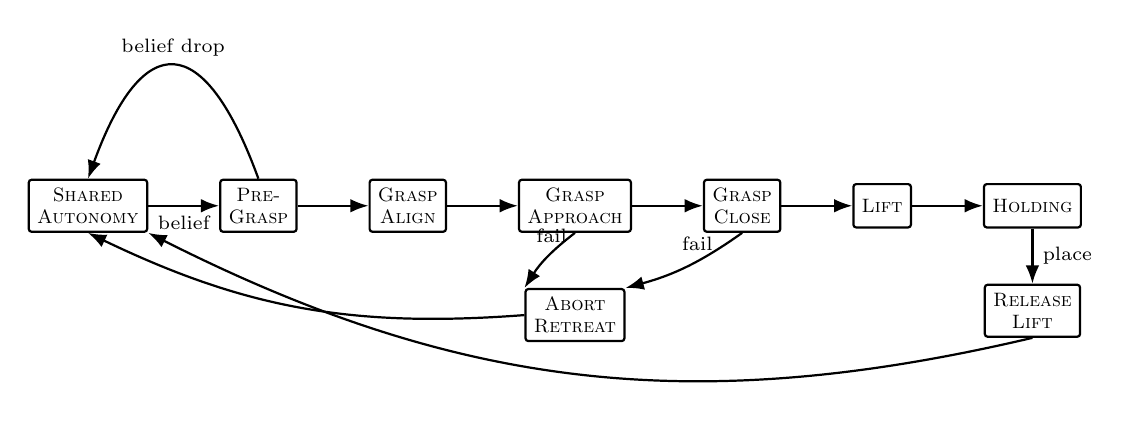
\begin{tikzpicture}[
  font=\scriptsize,
  state/.style={draw, rounded corners=1pt, align=center, inner sep=3pt, minimum height=5.5mm, fill=white},
  node distance=4mm and 9mm, >=Latex, every path/.style={thick}]
\node[state] (sa) {\textsc{Shared}\\\textsc{Autonomy}};
\node[state, right=of sa] (pg) {\textsc{Pre-}\\\textsc{Grasp}};
\node[state, right=of pg] (al) {\textsc{Grasp}\\\textsc{Align}};
\node[state, right=of al] (ap) {\textsc{Grasp}\\\textsc{Approach}};
\node[state, right=of ap] (cl) {\textsc{Grasp}\\\textsc{Close}};
\node[state, right=of cl] (li) {\textsc{Lift}};
\node[state, right=of li] (ho) {\textsc{Holding}};
\node[state, below=7mm of ap] (ab) {\textsc{Abort}\\\textsc{Retreat}};
\node[state, below=7mm of ho] (rl) {\textsc{Release}\\\textsc{Lift}};
\draw[->] (sa) -- node[below]{belief} (pg);
\draw[->] (pg) -- (al);
\draw[->] (al) -- (ap);
\draw[->] (ap) -- (cl);
\draw[->] (cl) -- (li);
\draw[->] (li) -- (ho);
\draw[->] (ho) -- node[right]{place} (rl);
\draw[->] (ap.south) to[bend right=10] node[above, pos=0.4]{fail} (ab.north west);
\draw[->] (cl.south) to[bend left=10] node[above, pos=0.4]{fail} (ab.north east);
\draw[->] (ab.west) to[bend left=15] (sa.south);
\draw[->] (rl.south) to[bend left=20] (sa.south east);
\draw[->] (pg.north) to[out=110, in=70, looseness=2.4] node[above]{belief drop} (sa.north);
\end{tikzpicture}
\caption{Grasp lifecycle. Belief hysteresis gates \textsc{Pre-Grasp} entry/exit; the autonomous chain runs on the robot policy with boosted tracking and frozen belief; failures retreat and return control to the operator.}
\label{fig:fsm}
\end{figure}

\textbf{Commit and execution.} A button press (Section~\ref{sec:studyapparatus}) requests a grasp, granted only when the object-level belief $B_{\text{obj}}(o^{\star})$~\eqref{eq:objbelief} and the \emph{measured} gripper pose are both within entry tolerance of the goal standoff, each with hysteresis so noise cannot chatter the state. Reading the real pose rather than the reference forces the operator to bring the arm itself to the standoff before the grasp will trigger. From \textsc{Grasp-Align} to \textsc{Lift} the arm then follows the per-goal robot policy with tracking boosted (Section~\ref{sec:sched}) and belief, blending, and teleoperation suspended; any phase timeout aborts into a retreat that returns authority to the operator.

\textbf{The object in the collision model.} Until the operator commits, the target cylinder is an ordinary obstacle in the safety controller's collision model, and the arm is barred from touching it as it would be from a wall. The commit is a declaration of intent to interact, and only then is the gripper--cylinder barrier pair released: that pair alone, with every other pair still enforced. The release is a ramp rather than a switch: the pair's safety margin moves smoothly from its normal value to a small negative allowance over a short interval, so the barrier row and its multiplier never jump and QP feasibility is preserved. Once the fingers close, the cylinder is re-parented as a kinematic link of the arm, leaving the obstacle set and joining the protected chain to avoid the rest of the world as it is carried. Release reverses the sequence: the object is detached to the world frame at its placed pose, where later grasp goals for it resolve, and re-enters the collision model through the same ramp, the gripper first backing off a measured clearance so that real separation exists before the barrier is fully active again. Across this whole cycle the barrier stays continuous, so the forward-invariance guarantee of Section~\ref{sec:cbf} holds during the grasp and release motions, not only before and after them. A graspable object is thus a conditionally active obstacle whose activation and deactivation are themselves executed under the barrier.

%───────────────────────────────────────────────────────────────────────────────
\section{Haptic interface: device model and force rendering}
\label{sec:teleop}

The operator commands the robot through a Haption Desktop 6D Compact, a six-degree-of-freedom impedance-type haptic interface: it measures handle motion and renders a commanded wrench on the handle. This section gives the device model, the two command mappings that turn handle motion into an arm reference, and the force laws that determine every wrench rendered on the handle, with and without assistance.

\subsection{Device frame and driver-side wrench}
\label{sec:device}

\textbf{Frame convention.} The device base frame and the robot base frame differ by a pure $180^{\circ}$ rotation about the vertical axis, so $\Phi = R_z(\pi) = \operatorname{diag}(-1,-1,1)$ simply flips the sign of the $x$- and $y$-components of any 3-vector (linear or axial), leaving the vertical component unchanged:
\begin{equation}
v^{\text{robot}} = \Phi\, v^{\text{dev}},
\qquad
F^{\text{dev}} = \Phi\, F^{\text{robot}},
\label{eq:flip}
\end{equation}
and because flipping twice returns the original vector, $\Phi$ undoes itself, so the same flip converts a velocity device $\to$ robot and a wrench robot $\to$ device: one formula, both directions.

\textbf{Viscous damping.} Every rendered wrench, in every condition, carries a constant viscous damper $(-K_d^{\text{lin}} v_h,\, -K_d^{\text{ang}} \omega_h)$ opposing handle motion, with $v_h$ and $\omega_h$ the handle linear and angular velocity. A damper is velocity feedback: it is passive only if the opposing wrench is applied in the same tick in which the velocity is measured, so it is computed at the device driver, within the tick, and added on top of whichever wrench the active force law supplies.

\textbf{Rate limiting.} The commanded wrench is also slew-limited between successive ticks,
\begin{equation}
\| F_k - F_{k-1} \| \le \dot{F}_{\max}\,\Delta t,
\qquad
\| \tau_k - \tau_{k-1} \| \le \dot{\tau}_{\max}\,\Delta t,
\label{eq:slew}
\end{equation}
where $F_k, \tau_k$ is the commanded force and torque at tick $k$, and $\dot F_{\max}, \dot\tau_{\max}$ are the maximum allowed rates of change: each new $F$ (respectively $\tau$) must land within a ball of radius $\dot F_{\max}\Delta t$ (respectively $\dot\tau_{\max}\Delta t$) around the previous command, not within a per-axis box, so a transition between force laws keeps its direction rather than skewing axis by axis as each component saturates on its own. The limiter is applied before the damper, so the damper's same-tick passivity is untouched. It is a rate limiter and not a low-pass filter by design: transparent to any signal changing slower than its bound, where a filter would lag every genuine force (Section~\ref{sec:filtering}). The angular slew bound $\dot\tau_{\max}$ has a hard floor set by the fastest legitimate signal in the system: the vibrotactile cues of Section~\ref{sec:columnbase}, a torque whose sign reverses every tick.

\subsection{Clutch mode --- position control}
\label{sec:clutchmode}

Clutch mode is position-control teleoperation with indexing. The handle twist is integrated into a pose reference,
\begin{equation}
p_{\text{ref}} \leftarrow p_{\text{ref}} + \Phi\, v_h\,\Delta t,
\qquad
R_{\text{ref}} \leftarrow \exp_3\!\bigl(\Phi\,\omega_h\,\Delta t\bigr)\, R_{\text{ref}},
\label{eq:clutchint}
\end{equation}
and published with the feed-forward twist consumed by the CLF row~\eqref{eq:clf}. While the clutch is held the reference is frozen and a zero twist is published, so the operator repositions the hand freely and a bounded device yields an unbounded workspace. The map is unscaled: workspace extension comes entirely from indexing, so hand and gripper displacements correspond one to one and the operator's kinaesthetic calibration transfers directly to fine manipulation. The integration anchor is the measured end-effector pose, re-captured on every arm switch and at the end of every autonomous phase, so teleoperation always resumes from where the robot physically is --- no jump, whatever the autonomous phase did.

\subsection{Joystick mode --- velocity control}
\label{sec:joystick}

Joystick mode is an alternative teleoperation mapping whose advantage is structural and holds for any device or robot: because the robot is commanded a velocity rather than an integrated position, no clutch is needed to reach the full workspace. The only persistent force on the handle is a centring spring toward a home pose (Section~\ref{sec:columnbase}), and intent is read purely as displacement from home. Releasing the handle recentres it, which is exactly a zero command. The two modes are the two classical families of master kinematic mapping, position control and rate control~\cite{kim1987comparison}, and constitute the control-mode factor of Section~\ref{sec:study}.

With the radial deadband operator
\begin{equation}
\operatorname{db}_{\varepsilon}(d) \;=\;
\begin{cases}
0, & \|d\| \le \varepsilon,\\[2pt]
\dfrac{\|d\|-\varepsilon}{\|d\|}\, d, & \|d\| > \varepsilon,
\end{cases}
\label{eq:db}
\end{equation}
a shrink of the displacement magnitude with direction preserved and continuous at its boundary, so that diagonal commands are not distorted as they are by per-axis deadbands, the commanded twist is proportional to the displacement past the deadband, lightly damped by the handle velocity, magnitude-clamped, and frame-flipped:
\begin{equation}
\begin{aligned}
v_{\text{user}} &= \Phi\,\operatorname{clamp}_{V_{\max}}\!\Bigl(K_t\,\operatorname{db}_{\varepsilon_{\text{lin}}}\!\bigl(p_h - p_{\text{home}}\bigr) \;-\; c_v\, v_h\Bigr),\\
\omega_{\text{user}} &= \Phi\,\operatorname{clamp}_{\Omega_{\max}}\!\Bigl(K_r\,\operatorname{db}_{\varepsilon_{\text{ang}}}\!\bigl(\log_3(R_h R_{\text{home}}^{\top})\bigr) \;-\; c_\omega\, \omega_h\Bigr),
\end{aligned}
\label{eq:jtwist}
\end{equation}
with the damping active only outside the deadband, so a handle resting or settling near home commands exactly zero. The deadband is sized above the centring spring's settling precision, so residual settling motion is never read as input.

The home position is fixed; the home orientation tracks the gripper, so that a handle at rest always means ``hold the current gripper orientation'':
\begin{equation}
R_{\text{home}} \;=\; \exp_3\!\Bigl(\tfrac{1}{s_r}\,\Phi \log_3\!\bigl(R_{\text{EE}}\,\bar{R}_{\text{arm}}^{\top}\bigr)\Bigr)\, R_0,
\label{eq:homerot}
\end{equation}
where $R_0$ is the neutral handle orientation, $\bar{R}_{\text{arm}}$ a per-arm gripper reference captured once at that arm's first activation and never re-anchored, and $s_r > 1$ compresses the gripper's excursion into the device's narrower, unevenly-ranged rotational workspace, the binding constraint on the hand-to-gripper map. The compression applies to the home pose only, never to the commanded twist. Because~\eqref{eq:homerot} is recomputed every tick, including while teleoperation is suspended, the home stays synchronised with the gripper and no state transition produces a jump; the same live home pose is the spring target of Section~\ref{sec:columnbase} and the zero point of~\eqref{eq:jtwist}.

Without blending the twist is integrated into a latched reference whose lead over the end-effector is bounded by projection,
\begin{equation}
\|p_{\text{ref}} - p_{\text{EE}}\| \le L_{\text{lin}},
\qquad
\bigl\|\log_3\!\bigl(R_{\text{ref}} R_{\text{EE}}^{\top}\bigr)\bigr\| \le L_{\text{ang}},
\label{eq:latchlead}
\end{equation}
so the reference cannot run away while the arm saturates against a constraint, and on release the arm catches up by at most the cap. With blending the pure user twist is passed to the arbitration law~\eqref{eq:blend} with the live end-effector pose as the belief anchor, $T_{\text{user}} \equiv T_{\text{EE}}$.

\subsection{Force rendering}
\label{sec:rendering}

Every wrench rendered on the handle is the superposition of a base layer, fixed by the control mode, and an assistance layer, fixed by the condition, with two invariants that hold in every condition: the superposed wrench is proportionally rescaled whenever its magnitude exceeds the authority cap $(F_{\text{cap}}, \tau_{\text{cap}})$, preserving direction and layer proportions so that the autonomy can never overpower the operator, and the published wrench is clipped to the device envelope.

The two columns are constructed as duals of one another, so that the assistance factor is compared on equal footing rather than against two unrelated baselines. Each column has one base force whose role is to restore the device to its rest relation with the robot. In the joystick column a centring spring returns the handle to the deadzone, where the commanded twist is zero; in the clutch column a coupling force --- the position-error feedback of a position--position bilateral scheme~\cite{hokayem2006bilateral}, which synchronises handle and robot --- draws the handle, and with it the integrated reference, back toward the robot's actual pose. Each column likewise keeps the operator's wrist aware of the gripper's orientation, without which neither mapping is usable at the wrist: the joystick home orientation tracks the gripper continuously~\eqref{eq:homerot}, so that a handle at rest means ``hold the current gripper orientation'', and the clutch column renders, whenever the clutch is held, an alignment torque that turns the handle toward the gripper~\eqref{eq:aligntorque}. And in both columns the guidance force of Section~\ref{sec:guidance} is rendered against that same base force: to follow the guidance the operator moves with it against the spring or the coupling, and to refuse it they move against both. The assistance is thus measured in the same currency in both columns --- as a fraction of the force that holds the device back --- which is what lets a difference between the columns be attributed to the mapping rather than to the feel of the assistance.

\subsection{Base force per column}
\label{sec:columnbase}

\textbf{Clutch column.} The base layer is the coupling force of the position--position scheme, a tether along the robot's tracking error, so the operator feels how far the arm lags its reference:
\begin{equation}
F_{\text{sync}}^{\text{lin}} = K_p^{s}\,\Phi\bigl(p_{\text{EE}} - p_{\text{ref}}\bigr),
\qquad
\tau_{\text{sync}} = K_R^{s}\,\Phi \log_3\!\bigl(R_{\text{EE}}\,R_{\text{ref}}^{\top}\bigr),
\label{eq:fsync}
\end{equation}
with no damping of its own, viscosity being supplied once by the driver-side damper of Section~\ref{sec:device}. The tether target is the published arm reference, which under blending is the blended reference --- the gripper the operator is actually watching.

While the clutch is held the tether is released and the rendered wrench carries an orientation-alignment torque alone: the operator repositions the hand freely in translation while the wrist is drawn into alignment with the gripper. The target is a difference referred to two anchors, not an absolute orientation. Writing $R_{\text{EE},0}$ for the pinned gripper orientation and $R_h$ for the live handle orientation,
\begin{equation}
\delta \;=\; \log_3\!\bigl(R_{\text{EE}}\,R_{\text{EE},0}^{\top}\bigr),
\qquad
R_{\text{target}} \;=\; \exp_3\!\bigl(\Phi\,\delta\bigr)\, R_0,
\label{eq:clutchalign}
\end{equation}
with the anchors $R_{\text{EE},0}$ and $R_0$ pinned once, at the end of startup homing (Section~\ref{sec:homing}), to the live gripper orientation and the neutral handle orientation. Pinning is mandatory: the gripper's and the handle's zero orientations are unrelated, so only differences transfer between the frames, and position control integrates orientation purely incrementally through~\eqref{eq:clutchint}. Mapping the rotation \emph{vector} through $\Phi$, rather than forming a matrix product across frames and repairing the torque afterwards, is what keeps the result a genuine rotation in the destination frame. The torque is a rotational spring on the residual $e_a = \log_3\!\bigl(R_{\text{target}}\,R_h^{\top}\bigr)$, saturated on its magnitude with its axis preserved,
\begin{equation}
\tau_{\text{align}} \;=\; M_a \tanh\!\Bigl(\frac{K_a\,\| e_a \|}{M_a}\Bigr)\,\frac{e_a}{\| e_a \|},
\label{eq:aligntorque}
\end{equation}
with $K_a$ the angular stiffness and $M_a$ the torque bound; a per-component saturation would distort the axis and break restorativeness, and a hard clip would turn the spring into a bang-bang law that self-excites into a limit cycle. The torque fades to zero within a margin of any device joint limit. Two vibrotactile cues complete the column, both a flat torque of fixed small amplitude whose sign reverses every tick, present exactly while their trigger holds: one while any device joint sits within a margin of its limit, one throughout autonomous grasp execution, during which the handle is additionally drawn to follow the end-effector.

\textbf{Joystick column.} The base layer is a centring spring toward the live home pose~\eqref{eq:homerot}:
\begin{equation}
F_{\text{home}} = K_P\bigl(p_{\text{home}} - p_h\bigr),
\qquad
\tau_{\text{home}} = K_R \log_3\!\bigl(R_{\text{home}}\,R_h^{\top}\bigr).
\label{eq:fhome}
\end{equation}
Through the gripper-tracking home orientation this is orientation synchronisation, while deliberately rendering no end-effector position tether --- coupling a robot-state force onto the handle whose displacement is then re-read as intent is the loop joystick mode exists to break. Its magnitude therefore differs from the clutch tether by design: the two frameworks define their base feedback differently, and that difference is part of the manipulated factor. The same vibrotactile cue signals the handle being outside either deadband, so the operator always feels when a command is being impressed, and signals autonomous grasp execution; no follow force accompanies the latter.

\subsection{Guidance force}
\label{sec:guidance}

In the assistive-feedback conditions the inferred intent is rendered as a feed-forward velocity-field force, a guidance virtual fixture~\cite{rosenberg1993virtual,abbott2007haptic}. The belief-weighted blend of the user-frame policies, the same weighting as in~\eqref{eq:blend}, is mapped into the device frame and saturated,
\begin{equation}
v_{\text{field}} \;=\; \Phi\!\sum_{k \in \mathcal{G}_{\text{act}}} b_k\, \pi_k^{\text{user}},
\qquad
F_{\text{guide}} \;=\; g \cdot
\begin{bmatrix}
M_F \tanh\!\bigl(D_F\, v_{\text{field}}^{\text{lin}} / M_F\bigr)\\[2pt]
M_\tau \tanh\!\bigl(D_\tau\, v_{\text{field}}^{\text{ang}} / M_\tau\bigr)
\end{bmatrix},
\label{eq:fguide}
\end{equation}
low-pass filtered for $C^0$ continuity across belief transitions. The gain $g \in [0,1]$ is the product of two smoothstep gates, identical in every guidance condition of both control modes:
\begin{equation}
g \;=\; \sigma\!\bigl(b_{\max};\, c_{\text{lo}}, c_{\text{hi}}\bigr)\,\cdot\,
\sigma\!\Bigl(\tfrac{d_{\text{far}} - \|p_{\text{ref}} - p_{g^{\star}}\|}{d_{\text{far}} - d_{\text{near}}};\, 0, 1\Bigr),
\qquad
\sigma(x; a, b) = 3u^2 - 2u^3,\;\; u = \operatorname{clip}\!\bigl(\tfrac{x-a}{b-a}, 0, 1\bigr).
\label{eq:guidegate}
\end{equation}
The confidence gate acts on the active-goal posterior $b_{\max} = \max_k b_k$ rather than on a peakedness measure such as normalised entropy, which is goal-count dependent; gating on $b_{\max}$ lets every condition share one belief function and one set of margins. The proximity gate silences guidance until the operator has brought the reference close enough for the goal manifold to be stable.

Three properties of~\eqref{eq:fguide} are structural. It is feed-forward, not velocity feedback: the form $D\,(v_{\text{field}} - v_{\text{handle}})$ is a virtual damper whose coefficient, at useful force levels, far exceeds what an impedance loop at $f_{\text{dev}}$ can render passively~\cite{colgate1994factors}; dropping the handle-velocity term makes the guidance a bias that shifts the equilibrium of the column's base spring, stability is recovered from the device's own dissipation, and the force still vanishes at the goal since $\pi_k \to 0$ there. The gain $g$ is applied after the saturation, so it reads directly as a fraction of the guidance authority. And in the joystick column the saturations are tied to the deadzone-exit force, the force needed to push the resting handle exactly to the deadband boundary,
\begin{equation}
M_F = \kappa\,\sigma_{\text{lin}}\, K_P\, \varepsilon_{\text{lin}},
\qquad
M_\tau = \kappa\,\sigma_{\text{ang}}\, K_R\, \varepsilon_{\text{ang}},
\qquad
\kappa\,\sigma_{(\cdot)} < 1,
\label{eq:kappacal}
\end{equation}
where $\kappa \in (0,1)$ is the deadzone-exit fraction and $\sigma_{\text{lin}}, \sigma_{\text{ang}} > 1$ per-channel trims. The constraint $\kappa\,\sigma_{(\cdot)} < 1$ is what keeps the guidance a strict bias: below unity it can never push the handle out of the deadband on its own, so the operator remains the sole initiator of motion. In the clutch column the saturations are absolute, sized against the sync-tether landscape (Appendix~\ref{app:config}).

%───────────────────────────────────────────────────────────────────────────────
\section{Head perception and the camera-derived safety world}
\label{sec:head}

The 7-DOF head carries an RGB-D camera and serves two roles: framing the operator's active hand during teleoperation, and building the collision world autonomously.

\subsection{Active-arm visual servoing (teleoperation)}
\label{sec:headtrack}

During teleoperation the head keeps the operator's active hand framed, tracking the grasp frame of the active gripper --- the same frame the safety QP, the belief estimator, and the grasp state machine treat as the hand. The head is driven by its own QP over the seven head-joint velocities and three task-slack variables, sharing no decision variable with the arm controller. With the hand inside the field of view, a 2.5D interaction-matrix formulation~\cite{malis1999,chaumette2006} maps pixel-plus-depth error to a camera twist through one relaxed equality row, with barrier rows holding the hand clear of the image edges; with the hand outside the field of view, a look-at law rotates the optical axis onto the hand direction. The rate at which the visual error is driven down is set jointly by the per-joint velocity cap of the joint-limit rows and the servo gain,
\begin{equation}
\dot{s} \;=\; \min\!\bigl(\qdot_{\max},\; \lambda_v\,\|e\|\bigr),
\label{eq:headvel}
\end{equation}
with $e$ the task error and $\lambda_v > 0$ the gain that sets the equality row's right-hand side $-\lambda_v e$: flat at $\qdot_{\max}$ for $\|e\| > \qdot_{\max}/\lambda_v$ and exponential at rate $\lambda_v$ below it, so the cap owns the far field and the gain the near field. Redundancy not spent on tracking is shaped by the same inverse-square joint-limit potential as the arm posture task (Section~\ref{sec:posture}), clamped at a fraction of the velocity cap so the field can never claim the whole velocity budget; near a bound the field and the joint-limit box push the same way. Soft cost terms additionally keep the image upright, lean the chain toward the active side, and orbit the viewpoint toward the gripper's approach axis, each gated so that it can neither fight acquisition nor override the equality and barrier rows. An active-arm switch first retracts the head to a compact home configuration under the barriers alone, so re-entry into tracking never begins from a stretched chain.

\textbf{Head-vs-arm collision barrier.} The safety QP carries the head chain as a quasi-static obstacle, but its dynamic margin~\eqref{eq:dsafe} thickens with the arm's own joint-velocity norm only, so a moving head acts on that barrier as an unmodelled disturbance. The head QP supplies the symmetric half from the arms' own barrier: the SoftMin aggregation of~\eqref{eq:softmin} is taken over $\mathcal{P}(\text{head})$, the active pairs that touch a head capsule, and the head QP appends
\begin{equation}
\bigl[J_{\text{soft},\text{head}}(q)\bigr]_{\mathcal{H}}\,\qdot_{\mathcal{H}}
\;\ge\;
-\,\gamma_{\text{head}}\,\Bigl(h_{\text{soft},\text{head}}(q) - \bigl(d_{\text{safe},\text{head}} + d_{\text{extra}}\bigr)\Bigr),
\label{eq:headcbf}
\end{equation}
where $\mathcal{H}$ is the index set of the head-chain joints within the full velocity vector and $[\,\cdot\,]_{\mathcal{H}}$ the matching column slice, $\qdot_{\mathcal{H}}$ the head QP's joint velocities, $\gamma_{\text{head}} < \gamma_{\text{cbf}}$ the head barrier gain, $d_{\text{safe},\text{head}} = d_0 + k_v\,\|\qdot_{\mathcal{H}}^{-}\|$ the head dynamic margin --- of the form~\eqref{eq:dsafe} but driven by the head velocity commanded on the previous tick, precisely the term the arm-side margin lacks --- and $d_{\text{extra}} > 0$ a fixed additional clearance on the head side only. With a lower gain and an extra margin, the head brakes sooner and more softly than the arm for the identical encounter, so a close call is paid for in camera-tracking performance rather than in arm task performance; the arm's own barrier on the same pair is untouched. If the appended row is infeasible against the joint-limit box, the head is commanded zero velocity: it freezes rather than colliding.

\subsection{Autonomous scene perception and the frozen snapshot}
\label{sec:convergence}

Independently of teleoperation, the head can build the collision world of Section~\ref{sec:task} from its own depth stream. The table plane is fitted by RANSAC~\cite{fischler1981ransac}, the points above it are clustered, and each cluster's rim is fitted by a circle to give the cylinder's centre, radius, and height; estimates are fused over time, and each object carries an \emph{arc coverage} recording which sectors of its circumference have been observed. Head motion is led by perception: fixation targets are chosen to raise the coverage of the least-covered object, frames are fused only while the head is settled, and the policy is bounded by a time budget.

The estimate is handed to the safety controller only when it has demonstrably stopped changing, by a criterion that needs no ground truth. Convergence requires every expected object present above a confidence floor and an arc-coverage floor $c_{\min}$, so that a geometrically insufficient view can never start the clock, and an oscillation-amplitude lock over a sliding window $\mathcal{W}$ of settled frames of duration $T_w$,
\begin{equation}
\max_{t \in \mathcal{W}} \bigl\|c(t) - \bar{c}_{\mathcal{W}}\bigr\| \le \varepsilon_{\text{pos}},
\qquad
\max_{t \in \mathcal{W}} \bigl|r(t) - \bar{r}_{\mathcal{W}}\bigr| \le \varepsilon_{\text{dim}},
\label{eq:amplock}
\end{equation}
with $c(t)$ and $r(t)$ each object's centre and radius, $\bar{c}_{\mathcal{W}}, \bar{r}_{\mathcal{W}}$ their window means, and $\varepsilon_{\text{pos}}, \varepsilon_{\text{dim}}$ the admitted bands; any head-motion frame clears the window, so motion time is never credited as stability. An amplitude band over a window captures slow drift and fast wobble in one frame-rate-independent test, which a per-frame drift counter cannot, since a static but wrong viewpoint passes it trivially. On convergence the estimate is frozen and published once as a latched snapshot --- table box and cylinders, each radius conservatively inflated --- which replaces the declared world as the safety controller's collision model, with everything downstream unchanged. The world is deliberately not updated per tick: a moving obstacle set would make the barrier non-stationary and void the forward-invariance argument of Section~\ref{sec:cbf}.

%───────────────────────────────────────────────────────────────────────────────
\chapter{Experiments and results}
\label{ch:exp}

\section{Setup of the experiments}
\label{sec:study}

The system is the apparatus of a user study run on the physical robot. The design is a $2\times3$ matrix crossing the teleoperation mapping with the assistance strategy:
\begin{itemize}[nosep]
\item \textbf{Control mode}, two levels --- \textsc{clutch}, position control with indexing (Section~\ref{sec:clutchmode}), and \textsc{joystick}, spring-centred velocity control (Section~\ref{sec:joystick});
\item \textbf{Assistance strategy}, three levels --- \emph{F}, the guidance force~\eqref{eq:fguide} rendered on the handle; \emph{B}, reference-level arbitration~\eqref{eq:blend} of the user twist with the belief-weighted policy; and \emph{FB}, both together.
\end{itemize}
This yields six conditions (Table~\ref{tab:cells}). The two channels are orthogonal by construction: F acts only on the handle and never modifies the reference; B acts only on the reference and is never rendered on the handle. Consequently the combined level is the exact superposition of the two single-channel levels --- the guidance wrench under FB is identical to the one under F, and adding B changes only \emph{which} reference the base tether tracks, not the rendered assistance law. The two off-diagonal conditions, \textsc{clutch} with B alone and \textsc{joystick} with F alone, each pair a control mode with its non-native channel --- the clutch framework was conceived around haptic feedback, the velocity joystick around automatic blending --- and are included to complete the matrix rather than as recommended operating points. Each control mode is also implemented with neither channel active, so the system realises eight configurations in all; the two unassisted ones are used for familiarisation and as a reference trace, and are excluded from the study matrix. The exclusion is a stated assumption rather than an oversight: that assisted teleoperation outperforms unassisted teleoperation on objective task metrics is already established for manipulation, and measured with the same task run both ways (Section~\ref{sec:sota-haptic-fixtures})~\cite{bettini2004vision}. Re-establishing it here would spend participant time on a settled comparison. The question this design does ask --- which channel, under which mapping, and whether the two compose --- is not answered by that literature, so every one of the six conditions contributes to it.

\begin{table}[b]
\centering\footnotesize
\begin{tabular}{@{}lccp{4.6cm}p{4.2cm}@{}}
\toprule
Condition & F & B & Operator feels & Arm reference written by \\
\midrule
\textsc{clutch} guided feedback  & \checkmark & --     & tether $+$ guidance bias & teleop (integrated pose) \\
\textsc{clutch} guided blending  & --     & \checkmark & tether (to the blended reference) & blending layer \\
\textsc{clutch} full guidance    & \checkmark & \checkmark & tether $+$ guidance bias & blending layer \\
\addlinespace[2pt]
\textsc{joystick} guided feedback & \checkmark & --     & spring $+$ guidance bias & teleop (latched twist integr.) \\
\textsc{joystick} guided blending & --     & \checkmark & homing spring $+$ cues & blending layer \\
\textsc{joystick} full guidance   & \checkmark & \checkmark & spring $+$ guidance bias & blending layer \\
\bottomrule
\end{tabular}
\caption{The six study conditions ($2$ control modes $\times$ $3$ assistance strategies). ``Cues'' are the vibrotactile signals of Section~\ref{sec:columnbase}; the guidance bias is~\eqref{eq:fguide}; the blending layer is the arbitration of Section~\ref{sec:blend}.}
\label{tab:cells}
\end{table}

Fairness across the matrix is treated as a first-class design feature, enforced by three mechanisms:
\begin{enumerate}[nosep]
\item \textbf{A single-value policy for shared building blocks.} Every mechanism appearing in more than one condition exists with exactly one parameterisation. Identical across all six conditions: the startup homing phase (Section~\ref{sec:homing}), the driver-side viscous damper (Section~\ref{sec:device}), the single vibrotactile cue design (Section~\ref{sec:columnbase}) --- one amplitude, one waveform, one tick period behind every cue, the joint-limit, out-of-deadband, and autonomous-grasp buzzes alike --- and the authority cap and the device clip. Identical within a column: the clutch sync tether~\eqref{eq:fsync} across the three clutch conditions, and the centring spring~\eqref{eq:fhome} across the three joystick conditions. Identical wherever the mechanism is active: the guidance gates~\eqref{eq:guidegate} in each F condition of \emph{both} modes, the guidance weights within each column, and the blending law with its authority parameters in each B condition. A measured difference between two conditions can therefore only be attributed to the manipulated factors.
\item \textbf{A startup condition guard.} The active condition triple is a single, centralised selection; every teleoperation node and force manager asserts at startup that it is the correct node for the selected condition and refuses to run otherwise. A mis-launched pairing fails loudly instead of silently running the wrong strategy --- protecting the integrity of a session's condition assignment.
\item \textbf{A single inference and safety stack.} Belief estimation, goal manifolds, policies, the grasp state machine, and the QP safety controller are byte-identical across all six conditions; a condition changes only the operator-input mapping and the rendered assistance.
\item \textbf{A no-initiation invariant.} Assistance modulates ongoing operator action but is calibrated never to act alone: blending suspends itself whenever the commanded twist drops below the stillness thresholds (Section~\ref{sec:blend}), and joystick-column guidance cannot push a resting handle past the deadband~\eqref{eq:kappacal}. In every condition, holding the handle still holds the robot still.
\end{enumerate}
Two asymmetries remain by design and are declared rather than equalised: the joystick base force is a \emph{homing} spring while the clutch base force is an \emph{error-tracking} tether (equalising their magnitudes would compare the wrong quantity --- each framework mandates its own base feedback, Section~\ref{sec:columnbase}); and the guidance saturation is absolute in the clutch column but deadzone-exit-calibrated in the joystick column~\eqref{eq:kappacal}, since each column's guidance must be commensurate with its own base-force landscape. Both are properties of the control-mode factor itself.

\subsection{Task and workspace}
\label{sec:studyworld}

Each participant works through two scenarios under every assigned condition. The two are chosen to differ in one structural respect --- whether the task \emph{requires} the arms to cooperate --- while keeping the object set, the grasp vocabulary, and the delivery-to-a-station goal common to both. This scenario factor is crossed with, and orthogonal to, the assistance factorial of Table~\ref{tab:cells}: assistance that helps a single arm run its own errand need not be the assistance that helps two arms hand an object between them.

\textbf{Relay scenario.} The task is a bimanual relay. Two cylinders rest on a table in front of the robot, and both must be delivered to a single station on a conveyor unit standing to the robot's right. A storage-rack shelf spans the table just above the cylinders and closes the overhead approach corridor, so every pick and every place at the table is a side grasp. The conveyor sits clear of the shelf, so its station admits a top approach, but only the right arm reaches it. The right arm can therefore pick its cylinder and carry it straight to the conveyor; the left arm cannot, and instead stages its cylinder on an intermediate handover disk on the table --- offset toward the robot's right so that it falls within both arms' reach --- from which the right arm relays it onward.

The coordination the task elicits is a property of the workspace geometry, not of an inserted obstacle. No divider stands between the two arms: the handover is forced purely by reach, because the delivery station lies where one arm alone can serve it. An operator who never hands over cannot finish the task. What is measured is therefore a response to the task itself rather than to an artificial barrier added to provoke it.

Both scenes also carry decorative industrial fixtures --- a perimeter fence, an overhead gantry, cabinets, pallets, and the conveyors' own frames and rollers. None of these carry collision geometry, and none enter the safety controller's world model; they give the operator visual context and nothing more. The barrier's forward-invariance guarantee (Section~\ref{sec:cbf}) is stated over the \emph{declared} collision model, so a fixture that is drawn but not declared lies outside that guarantee by construction. Each declared model contains only the table, the two cylinders, the scenario's own blocking structure --- the rack shelf with its supports, or the shield pane --- and one convex envelope per conveyor.

\textbf{Independent scenario.} The second scenario removes the coupling and adds an obstacle instead. A thin transparent safety shield stands between the robot and the table, spanning its full width so that no lateral window is left; each arm must therefore reach \emph{over} the shield to work. Two conveyor units flank the table, mirror-symmetric about the robot's sagittal plane, each carrying its own delivery station. Each arm picks the cylinder on its own side and delivers it to the station on that side: the errands are independent, symmetric, and concurrent, with no handover and nothing contested between the arms. Because the shield closes the low approach and leaves the overhead corridor open, every grasp here is a top grasp --- the complement of the relay scenario, where the shelf closes the overhead corridor and every grasp is a side grasp. Between them the two scenarios exercise both grasp manifolds of Section~\ref{sec:policies} and both the coordinated and the independent regimes of the bimanual controller.

Each scenario declares its placement stations as platforms --- the handover disk and the conveyor station in the relay scenario, the two mirrored conveyor stations in the independent one. Each is demandable by either arm while that arm holds a cylinder, and belief estimation together with guidance selects which platform is the active placement goal, exactly as they select among grasp goals (Section~\ref{sec:policies}). Like every platform, they are reference poses for the goal manifold and the guidance law alone, and none enters the collision model.

\subsection{Environment model and camera use}
\label{sec:studyenv}

Two facts about the environment fix what the study tests. First, the collision world in every study trial is the declared model of Section~\ref{sec:task}, loaded from the scenario's description file; the autonomous perception pipeline of Section~\ref{sec:convergence} is not in the loop, so no trial's safety depends on the camera's estimate of the scene. Second, the head is nonetheless active throughout: it runs the active-arm visual servoing of Section~\ref{sec:headtrack}, and its camera image --- a view that follows and zooms on the gripper being driven --- is the operator's primary view of the task. The camera thus serves the operator's perception, not the controller's.

The perception pipeline was validated separately on the physical robot. The head scanned a table carrying two cups; the table plane and both objects were recovered by the RANSAC-based estimator, and the frozen snapshot was loaded as the safety controller's collision model. Teleoperation and barrier-based obstacle avoidance were then exercised against that perceived model, confirming the pipeline end to end, from depth stream to enforced constraint.

\subsection{Apparatus and instrumentation}
\label{sec:studyapparatus}

A single bringup starts the simulator and the robot model, the robot's default arm and torso controllers, the mobile-base teleoperation, and three visualisation stations. The first is the operator's own station: it carries the head-camera image and a first-person view that follows one gripper. The second is a wide overview of the whole scene. The third is a first-person view following the other gripper, so an experimenter can watch the hand the operator is not driving at that moment. Each station renders a filtered robot description in which every link outside the two arm-and-gripper chains is dimmed to a translucent grey, so that the operator's sight line to the hands and the task is not blocked by the robot's own torso, base, and head. The filter acts at the description source --- it rewrites the model the visualiser loads --- because per-link transparency overrides applied inside the visualiser have no visual effect on this robot's meshes. Collision and inertial data are left untouched, and the unfiltered description stays available to every other consumer.

\textbf{Operator controls.} The two device buttons carry all discrete operator commands. The right button is the clutch: while held, the pose reference is frozen (Section~\ref{sec:clutchmode}) and, in blended conditions, reference blending is suspended so that hand repositioning neither moves the robot nor is read as intent (Section~\ref{sec:blend}). The left button is an event channel read by edge detection over a double-press window: a single press requests a grasp, a double press switches the active arm. Arm switching is decided in the shared-autonomy node alone, which publishes it and every other node follows, so no two nodes can disagree about which arm is being driven.

\textbf{Startup homing.}
\label{sec:homing}
Every session opens with a homing phase in which the only rendered wrench is a soft parking spring of the form of~\eqref{eq:fhome}, drawing the handle to a fixed neutral pose and faded in over a fixed interval, so that every participant begins from the same handle configuration; the spring is far softer than either column's operating spring, since the operator need not be holding the handle while it runs. The phase ends once the handle has held within position and orientation tolerances for a settle window, or after a timeout. Both teleoperation nodes suspend their output while it runs, so the homing motion is never fed to the robot, and the anchors of the clutch-hold alignment~\eqref{eq:clutchalign} are pinned at its end.

The safety controller and the shared-autonomy node run outside this bringup. Either can be restarted after a parameter change or a fault without tearing down and rebuilding the simulator --- which is what makes an eight-condition session practical to run.

\subsection{Data capture and questionnaire}
\label{sec:studydata}

Each trial is captured as a single time-stamped recording of the robot and telemetry topics, started and stopped from a small experimenter interface that also writes the trial's provenance --- participant, scenario, condition, a manually assigned success flag, and free-text notes. On save, the interface additionally launches that trial's offline analysis as a low-priority background job, so the per-trial dashboards and metrics are prepared without delaying the next trial.

The subjective instrument is administered once per condition, after the participant has attempted that condition on both scenarios, rather than once per trial; it therefore carries no scenario field. It is a short form: a trimmed subset of standard workload items~\cite{hart1988nasatlx} together with three human--robot-interaction items --- perceived control, trust~\cite{jian2000trust}, and comfort --- each on an ordinal scale. It is collected electronically, with the condition picked from a fixed list rather than typed, so the key that joins a response to its trials cannot be mistyped. All six conditions are surveyed; the unassisted configuration used for familiarisation is not.

\section{Results}
% TODO: to be written


%───────────────────────────────────────────────────────────────────────────────
\chapter{Discussion}
\label{ch:discussion}

\section{Summary of design choices and trade-offs}

\begin{itemize}[nosep]
\item \textbf{Per-arm CBF split over a shared row}: eliminates idle-arm coupling at the cost of losing global cross-arm margin sharing for non-inter-arm pairs --- acceptable since the inter-arm pairs still contribute to both rows. The per-arm dynamic margin~\eqref{eq:dsafe} closes the residual coupling channel.
\item \textbf{Normalised scalar CLF with a per-arm slack}: uniform constraint conditioning across error magnitudes; tracking degrades gracefully under conflict, safety never does.
\item \textbf{Measured-anchor rate damping over a slew-rate box}: gives the task-null wrist DOFs tick-to-tick memory anchored to the arm's physical state; a hard box provably risks infeasibility against a direction-switching CBF row. The weight is stall-scheduled per arm --- full only near convergence, relaxed at large error --- because a strong pull toward a near-zero measured velocity otherwise self-reinforces a freeze (Section~\ref{sec:rate}).
\item \textbf{Quasi-static head model on the arm side, a dynamic barrier on the head side}: the arm's barrier holds the head chain as a quasi-static obstacle, which keeps it out of the QP decision vector, and its dynamic margin responds to arm speed alone. The complementary guarantee is carried by the head controller, whose own barrier on the same chain pairs has a margin that does see the head's speed. That barrier is asymmetric --- half the arm's gain, plus an extra fixed clearance --- so a close encounter is paid for in camera-tracking performance rather than in arm task performance (Section~\ref{sec:headtrack}).
\item \textbf{Alignment-based authority over belief-gated authority}: belief selects the goal, alignment arbitrates control; opposition ramps autonomy authority to exactly zero and stillness suspends blending outright, so the operator always wins a direct conflict and assistance never initiates motion.
\item \textbf{Goal manifolds over fixed grasp poses}: only the task-required degrees of freedom are constrained and the operator's own anchor resolves the rest, so assistance never fights a choice the task is indifferent to. The free directions are stabilised structurally rather than by discrete locking: the top-grasp roll is resolved in closed form, with no candidate set and no hysteresis; the side-grasp azimuth is a confidence-ramped blend of two estimates whose degeneracies are disjoint, so one is always well posed; and both free directions are rate-bounded by a normalised direction filter. One discrete latch with distance-scaled hysteresis remains, on the side-grasp finger-orientation choice alone (Section~\ref{sec:policies}).
\item \textbf{Feed-forward guidance over velocity-field damping}: the $-v_{\text{handle}}$ feedback term is a virtual damper far beyond the $150$~Hz impedance passivity budget and would excite a limit cycle; the feed-forward form biases the base spring's equilibrium, is rendered stably by the device's own dissipation, and still vanishes at the goal (Section~\ref{sec:guidance}).
\item \textbf{Spring-centred joystick over force-tethered pose integration}: breaks the force $\to$ displacement $\to$ intent feedback loop structurally instead of tuning around it (Section~\ref{sec:joystick}).
\item \textbf{Deadzone-exit-calibrated guidance authority ($\kappa < 1$)}: guidance can bias but never autonomously drive --- the operator remains the sole initiator of motion in velocity mode~\eqref{eq:kappacal}.
\item \textbf{Driver-side damping and slew limiting}: a viscous damper is passive only when its wrench is applied in the tick the velocity was measured, so it is formed inside the device driver rather than returned across a process boundary from a force manager. The command slew limiter sits in the same place, bounding the magnitude of the commanded-wrench change vector across a mode switch so a transition keeps its direction instead of stepping axis by axis. It is a rate limiter, not a low-pass filter, so it stays transparent to any signal slower than its bound --- at the price of a hard floor on that bound, fixed by the fastest legitimate signal, the vibrotactile cue (Section~\ref{sec:device}).
\item \textbf{Delta-mapped clutch-hold alignment over an absolute map}: the gripper's and the handle's zero orientations are unrelated, so only orientation \emph{differences} transfer between the device and robot frames; an absolute map would assume the two zeros coincide and pull the handle toward a plausible but wrong pose. Referring that difference to two anchors pinned once, at the end of startup homing, is also what makes the servoed target reproducible from session to session (Section~\ref{sec:columnbase}).
\item \textbf{Single-value fairness policy across the study matrix}: every shared gain and gate exists with exactly one value across the six conditions, enforced by a startup condition guard; measured differences are attributable only to the manipulated factors (Section~\ref{sec:study}).
\item \textbf{Reference governor before the CLF}: preserves hard QP feasibility under arbitrarily aggressive teleoperation commands, without enlarging slack bounds or softening safety margins.
\item \textbf{Frozen perceived world over per-tick perception updates}: the camera-derived collision model is convergence-gated (Section~\ref{sec:convergence}) and then static, preserving the barrier's stationarity; re-scans are explicit events.
\item \textbf{No force sensing}: grasp confirmation is purely kinematic; the perception pipeline closes the world-modelling half of this gap (Section~\ref{sec:head}).
\end{itemize}

\chapter{Conclusions}
\label{ch:conclusions}
% TODO: to be written

\section*{Code availability}
The software described in this thesis is available in two repositories: the robot-side stack --- safety controller, shared autonomy, grasp lifecycle, and head perception --- at \url{https://github.com/Robertorocco/triago_control}, and the operator-side stack --- device driver, teleoperation modes, and force managers --- at \url{https://github.com/Robertorocco/haption_teleoperation}.


\appendix
\chapter{Configuration parameters}
\label{app:config}


All parameter values live in centralised configuration modules (one per subsystem) and are reported here, grouped by function. Symbols refer to the equations above.

\begingroup\footnotesize

\section{Control loop}
\begin{tabularx}{\linewidth}{@{}lllX@{}}
\toprule
Symbol & Name & Value & Meaning \\
\midrule
$f_{\text{ctrl}}$ & \texttt{CONTROL\_FREQ\_DEFAULT} & 150~Hz & safety-controller loop rate \\
--- & \texttt{PUBLISH\_EVERY\_N} & 2 & telemetry decimation \\
--- & \texttt{WATCHDOG\_TIMEOUT} & 0.5~s & stale reference $\Rightarrow$ freeze arm \\
--- & \texttt{ALPHA\_FILTER} & 0.5 & EMA coefficient, velocity reconstruction \\
\bottomrule
\end{tabularx}

\section{CLF / task tracking (Section~\ref{sec:clf}, Section~\ref{sec:sched})}
\begin{tabularx}{\linewidth}{@{}lllX@{}}
\toprule
Symbol & Name & Value & Meaning \\
\midrule
$\gamma$ & \texttt{GAMMA\_CLF\_DEFAULT} & 0.75 & CLF convergence rate (constant) \\
$\gamma_{\max}$ & \texttt{GAMMA\_MAX} & 1.2 & CLF rate for a frozen / autonomous-grasp arm \\
$W_{\text{task}}$ & \texttt{TASK\_WEIGHTS\_6D} & $\mathrm{diag}(10,10,10,0.5,0.5,0.5)$ & position:orientation $=20{:}1$ \\
$W_{\text{task}}^{\text{grasp}}$ & \texttt{TASK\_WEIGHTS\_6D\_GRASP} & $\mathrm{diag}(10,10,10,2,2,2)$ & precision phases, $5{:}1$ \\
$w_{\delta}^{\text{base}}, w_{\delta}^{\max}$ & \texttt{BASE/MAX\_WEIGHT\_SLACK} & 150.75 / 250 & slack-weight schedule range: base against a constraint, ceiling in free space \eqref{eq:slacksched} \\
$\beta$ & \texttt{BETA} & 0.2 & slack-schedule sensitivity \\
$\tau_{\lambda}$ & \texttt{SLACK\_FILTER\_TAU} & 0.15~s & shadow-price LPF (input stage) \\
$\tau_{w}$ & \texttt{WEIGHT\_SLACK\_FILTER\_TAU} & 0.2~s & slack-weight LPF (output stage) \eqref{eq:slacksched} \\
\bottomrule
\end{tabularx}

\section{CBF / collision (Section~\ref{sec:cbf})}
\begin{tabularx}{\linewidth}{@{}lllX@{}}
\toprule
Symbol & Name & Value & Meaning \\
\midrule
$\alpha_s$ & \texttt{ALPHA\_SOFTMIN} & 60 & SoftMin aggregation sharpness \eqref{eq:softmin} \\
$\gamma_{\text{cbf}}$ & \texttt{GAMMA\_CBF} & 0.70 & barrier class-$\mathcal{K}$ gain \eqref{eq:cbf} \\
$d_0$ & \texttt{D\_SAFE\_BASE} & 0.015~m & base safety margin \eqref{eq:dsafe} \\
$k_v$ & \texttt{K\_V\_SAFE} & 0.1~s & velocity margin horizon \eqref{eq:dsafe} \\
--- & \texttt{DISTANCE\_FILTER\_THRESHOLD} & 0.15~m & pair activation radius \\
$K$ & \texttt{K\_MAX\_PAIRS} & 60 & closest pairs kept per tick \\
--- & \texttt{CAPSULE\_RADIUS} & 0.06~m & default arm-capsule radius \\
\bottomrule
\end{tabularx}

\section{QP cost (Section~\ref{sec:posture}, Section~\ref{sec:rate}) and joint limits (Section~\ref{sec:jl})}
\begin{tabularx}{\linewidth}{@{}lllX@{}}
\toprule
Symbol & Name & Value & Meaning \\
\midrule
$\lambda$ & \texttt{DAMP} & 12 & joint-velocity damping; $2\lambda$ on a frozen arm's joints \\
$w_c$ & \texttt{W\_CENTER} & 0.96 & posture-field weight \\
$k_g$ & \texttt{K\_GRADIENT} & 0.07 & posture gradient gain \\
$v_{\max}^{\text{post}}$ & \texttt{V\_MAX\_POSTURE} & 1.0~rad/s & posture reference clamp \\
--- & \texttt{POSTURE\_GRASP\_SCALE} & 0.05 & posture scale in precision phases \\
--- & \texttt{POSTURE\_SCALE\_TAU} & 0.2~s & posture-scale ramp \\
$\rho$ & \texttt{RATE\_WEIGHT} & 50 & rate-damping weight, full: position error below the stall threshold and no autonomous grasp \\
--- & \texttt{RATE\_WEIGHT\_GRASP} & 20 & rate-damping weight, relaxed: autonomous grasp or large error \\
--- & \texttt{STALL\_ERR\_POS\_THRESH} & 0.10~m & position-error threshold switching $\rho_i$ \\
--- & \texttt{RATE\_DAMPING\_VS\_MEASURED} & true & measured anchor (Section~\ref{sec:rate}) \\
$k_p$ & \texttt{P\_GAIN\_LIMITS} & 1.8 & joint-limit braking gain \\
$b_0$ & \texttt{JOINT\_LIMIT\_BUFFER\_BASE} & 0.15~rad & base braking buffer \\
$k_b$ & \texttt{JOINT\_LIMIT\_K\_V} & 0.1~s & buffer velocity horizon \\
\bottomrule
\end{tabularx}

\section{Reference governor (Section~\ref{sec:governor})}
\begin{tabularx}{\linewidth}{@{}lllX@{}}
\toprule
Symbol & Name & Value & Meaning \\
\midrule
$V_{\max}^{\text{lin}}$ & \texttt{GOV\_V\_MAX\_LIN} & 0.20~m/s & reference linear speed cap \\
$V_{\max}^{\text{ang}}$ & \texttt{GOV\_V\_MAX\_ANG} & 0.3~rad/s & reference angular speed cap \\
$E_{\max}^{\text{pos}}$ & \texttt{GOV\_E\_MAX\_POS} & 0.30~m & position-error bound \\
$E_{\max}^{\text{ori}}$ & \texttt{GOV\_E\_MAX\_ORI} & 1.0~rad & orientation-error bound ($\sim$57$^\circ$) \\
$A_{\max}^{\text{lin}}$ & \texttt{GOV\_A\_MAX\_LIN} & 0.75~m/s$^2$ & linear acceleration cap \\
$A_{\max}^{\text{ang}}$ & \texttt{GOV\_A\_MAX\_ANG} & 3.0~rad/s$^2$ & angular acceleration cap \\
\bottomrule
\end{tabularx}

\section{Shared autonomy (Section~\ref{sec:sa})}
\begin{tabularx}{\linewidth}{@{}lllX@{}}
\toprule
Symbol & Name & Value & Meaning \\
\midrule
$W$ & --- & $\mathrm{diag}(10,10,10,2,2,2)$ & policy/belief twist metric \eqref{eq:policyqp},\eqref{eq:cost-belief} \\
$w_{\text{pos}}$ & --- & 0.1 & position-cost blend weight in the belief evidence \eqref{eq:cost-belief} \\
$K_p$ & --- & 0.5 & policy proportional gain \eqref{eq:vgeo} \\
$v_{\max},\omega_{\max}$ & --- & 0.1~m/s, 0.3~rad/s & robot-policy saturation \\
$v_{\max}^{u},\omega_{\max}^{u}$ & --- & 0.04~m/s, 0.10~rad/s & user--policy saturation \\
$\beta_0$ & --- & 0.04 & belief step size \eqref{eq:effgains} \\
$\alpha_0$ & --- & 0.995 & belief forgetting factor \eqref{eq:effgains} \\
$v_{\text{lo}}, v_{\text{hi}}$ & \texttt{BELIEF\_V\_LOW/HIGH} & 0.005 / 0.030~m/s & engagement ramp \eqref{eq:engagement} \\
$g_{\min}$ & --- & 0.05 & engagement floor \\
--- & \texttt{BELIEF\_WARMUP\_S} & 2.5~s (floor 0.25) & post-reset exploration window \\
$B_{\text{obj}}^{\text{ent}}, B_{\text{obj}}^{\text{stay}}$ & \texttt{BELIEF\_ENTER/STAY} & 0.90 / 0.75 & object-level belief hysteresis, \textsc{Pre-Grasp} entry / stay \eqref{eq:objbelief} \\
$\alpha_{\min},\alpha_{\max}$ & \texttt{ALIGN\_ALPHA\_MIN/MAX} & 0.2 / 0.8 & authority ramp \eqref{eq:alpha} \\
$v_{\text{still}},\omega_{\text{still}}$ & --- & 0.005~m/s, 0.05~rad/s & stillness gate: blend suspended below (Section~\ref{sec:blend}) \\
--- & \texttt{ALIGN\_ALPHA\_LPF\_COEFF} & 0.1 & authority LPF \\
$\tau_{\text{dir}}$ & \texttt{GOAL\_DIRECTION\_FILTER\_TAU} & 4.0~s & normalised-EMA time constant on the resolved free directions (side azimuth, top roll) (Section~\ref{sec:policies}) \\
--- & \texttt{SIDE\_STANDOFF\_FROM\_CENTER} & 0.03~m & side-grasp standoff from the cylinder axis \\
--- & \texttt{ORIENT\_LOCK\_NEAR/FAR} & 0.12 / 0.30~m & distance-scaled sticky-hysteresis ramp for the side-grasp finger-orientation candidate ($180^{\circ}$ apart); the top-grasp roll is resolved in closed form (Section~\ref{sec:policies}) \\
\bottomrule
\end{tabularx}

\section{Grasp lifecycle (Section~\ref{sec:grasp})}
\begin{tabularx}{\linewidth}{@{}lllX@{}}
\toprule
Symbol & Name & Value & Meaning \\
\midrule
--- & \texttt{POS/ANG\_ERR\_ENTER} & 0.040~m / 0.16~rad & staging gate, \textsc{Pre-Grasp} entry \\
--- & \texttt{POS/ANG\_ERR\_STAY} & 0.072~m / 0.224~rad & staging gate, stay (hysteresis) \\
--- & \texttt{ALIGN\_POS\_TOL}, \texttt{ALIGN\_ANG\_TOL} & 0.0209~m / 0.103~rad & tight standoff tolerance \textsc{Align} converges to before insertion \\
--- & \texttt{ALIGN\_CENTERING\_TOL} & 20.7~mm & lateral centring tolerance (insertion line to cylinder axis), \textsc{Align} \\
--- & \texttt{GRASP\_CBF\_MARGIN} & $-0.08$~m & gripper--cylinder pair envelop allowance during insertion \\
--- & \texttt{GRASP\_CONTACT\_DEPTH\_TOP/SIDE} & $-0.03$ / $-0.04$~m & gripper-box--cylinder overlap gating finger closure (top / side) \\
--- & \texttt{GRASP\_INSERTION\_TRAVEL\_TOP/SIDE} & 0.09 / 0.068~m & blind insertion travel from the standoff (top / side) \\
--- & \texttt{ALIGN\_TIMEOUT\_S}, \texttt{GRASP\_APPROACH\_TIMEOUT\_S} & 12 / 15~s & \textsc{Align} / \textsc{Approach} phase timeouts $\to$ \textsc{Abort-Retreat} \\
--- & \texttt{RELEASE\_RETREAT\_DISTANCE/VELOCITY} & 0.14~m, 0.10~m/s & post-release retreat: measured travel before authority returns, commanded speed \\
--- & \texttt{RELEASE\_RETREAT\_MAX\_S} & 3.5~s & post-release retreat timeout cap \\
--- & \texttt{ABORT\_RETREAT\_DISTANCE/VELOCITY} & 0.10~m, 0.05~m/s & failed-grasp retreat: measured travel, commanded speed \\
--- & \texttt{ABORT\_RETREAT\_MAX\_S} & 6.0~s & failed-grasp retreat timeout cap \\
\bottomrule
\end{tabularx}

\section{Head perception and world convergence (Section~\ref{sec:head})}
\begin{tabularx}{\linewidth}{@{}lllX@{}}
\toprule
Symbol & Name & Value & Meaning \\
\midrule
--- & \texttt{WORLD\_CONF\_MIN} & 0.85 & per-object confidence floor \\
$c_{\min}$ & \texttt{WORLD\_MIN\_ARC\_COVERAGE} & 0.55 & arc-coverage floor \\
$\varepsilon_{\text{pos}}$ & \texttt{WORLD\_CONVERGE\_POS\_AMP} & 1~mm & centre amplitude band \eqref{eq:amplock} \\
$\varepsilon_{\text{dim}}$ & \texttt{WORLD\_CONVERGE\_DIM\_AMP} & 1.5~mm & radius/height amplitude band \\
$T_w$ & \texttt{WORLD\_CONVERGE\_WINDOW\_S} & 1.0~s & amplitude-lock window \\
--- & \texttt{WORLD\_EXPECTED\_CYLINDERS} & 2 & objects required present \\
--- & \texttt{INTEGRATE\_VEL\_THRESH} & 0.04~rad/s & head-settled fusion gate \\
--- & \texttt{ACTIVE\_VISION\_TIME\_BUDGET\_S} & 45~s & scan/refine wall-clock cap \\
--- & \texttt{ACTIVE\_VISION\_PLATEAU\_EPS} & 0.01 (patience 6) & coverage-gain plateau test \\
--- & \texttt{ACTIVE\_VISION\_REFINE\_OFFSET} & 0.06~m & unseen-azimuth fixation offset \\
--- & \texttt{CYL\_RADIUS\_INFLATION} & 0~m & snapshot cylinder-radius inflation \\
\bottomrule
\end{tabularx}

\section{Head active-arm tracking (Section~\ref{sec:headtrack})}
\begin{tabularx}{\linewidth}{@{}lllX@{}}
\toprule
Symbol & Name & Value & Meaning \\
\midrule
$\lambda_v$ & \texttt{LAMBDA\_VISUAL} & 2.5 & visual-servo convergence gain, near field \eqref{eq:headvel} \\
$\qdot_{\max}$ & \texttt{MAX\_VELOCITY} & 0.20~rad/s & per-head-joint velocity cap, far field \eqref{eq:headvel} \\
--- & \texttt{TARGET\_DISTANCE} & 0.7~m & camera stand-off from the active hand \\
$\gamma_{\text{head}}$ & \texttt{GAMMA\_CBF\_HEAD} & 0.35 & head-vs-arm barrier gain ($\tfrac{1}{2}\gamma_{\text{cbf}}$) \eqref{eq:headcbf} \\
$d_{\text{extra}}$ & \texttt{D\_SAFE\_HEAD\_EXTRA} & 0.03~m & fixed extra clearance, head side only \eqref{eq:headcbf} \\
--- & \texttt{GAMMA\_FOV} & 5.0 & FOV barrier class-$\mathcal{K}$ gain \\
--- & \texttt{FOV\_MARGIN} & 50~px & image-edge distance triggering the FOV barrier \\
--- & \texttt{W\_SLACK\_PIXELS}, \texttt{W\_SLACK\_DEPTH} & $1.0$, $10^{4}$ & image-based task-slack weights (pixel, depth) \\
--- & \texttt{W\_SLACK\_PBVS} & $10^{4}$ & position-based (look-at) task-slack weight \\
--- & \texttt{JOINT\_WEIGHTS} & 5.0 & uniform per-joint velocity regularisation \\
$k_g^{\text{head}}$ & \texttt{K\_POSTURE\_GRADIENT} & 0.05 & head posture-field gradient gain \\
--- & \texttt{V\_MAX\_POSTURE} & 0.15~rad/s & head posture reference clamp (half the velocity cap) \\
--- & \texttt{K\_HOME} & 1.5~s$^{-1}$ & arm-switch homing joint-space servo gain \\
--- & \texttt{HOME\_TOL} & 0.12~rad & max-abs joint error ending the homing phase \\
--- & \texttt{HOME\_TIMEOUT\_S} & 5.0~s & homing-phase timeout \\
--- & \texttt{HOME\_Y\_BIAS} & 0.20~m & lateral home offset toward the tracked arm's side \\
--- & \texttt{LEAN\_FRACTION} & 0.6 & head-elbow lateral target as a fraction of the active hand's \\
--- & \texttt{K\_LEAN} & 1.5~s$^{-1}$ & chain-lean servo gain \\
--- & \texttt{APPROACH\_GATE\_ANGLE\_DEG} & $40^{\circ}$ & approach-alignment gate: fades out past this hand off-axis angle \\
--- & \texttt{TOP\_VIEW\_BIAS} & 0.3 & orbit-axis blend toward straight-overhead framing \\
--- & \texttt{K\_ROLL\_ALIGN} & 1.0~s$^{-1}$ & image up-righting servo gain \\
--- & \texttt{ROLL\_GATE\_ANGLE\_DEG} & $30^{\circ}$ & up-righting authority fades out past this hand off-axis angle \\
$f_{\text{head}}$ & \texttt{CONTROL\_HZ} & 50~Hz & head control-loop rate \\
\bottomrule
\end{tabularx}

\section{Teleoperation: device and control modes (Section~\ref{sec:teleop})}
\begin{tabularx}{\linewidth}{@{}lllX@{}}
\toprule
Symbol & Name & Value & Meaning \\
\midrule
$f_{\text{dev}}$ & \texttt{VIRTUOSE\_FREQUENCY} & 150~Hz & device server / teleop / force-manager rate \\
$T_{\text{dp}}$ & \texttt{DOUBLE\_CLICK\_WINDOW} & 0.5~s & left-button double-press window \\
--- & \texttt{K\_trans}, \texttt{K\_rot} & 1.0 & clutch motion scale (1:1, unscaled) \\
$\varepsilon_{\text{lin}}$ & \texttt{JOYSTICK\_DEADBAND\_LIN} & 0.03456~m & linear deadband ($\sim$3.5~cm) \eqref{eq:db} \\
$\varepsilon_{\text{ang}}$ & \texttt{JOYSTICK\_DEADBAND\_ANG} & 0.16330~rad & angular deadband ($\sim$9.4$^\circ$) \\
$K_t$ & \texttt{JOYSTICK\_K\_TRANS} & 1.6~s$^{-1}$ & twist gain, linear \eqref{eq:jtwist} \\
$K_r$ & \texttt{JOYSTICK\_K\_ROT} & 1.65~s$^{-1}$ & twist gain, angular \\
$c_v, c_\omega$ & \texttt{JOYSTICK\_DAMP\_LIN/ANG} & 0.225 / 0.075 & twist damping fractions \\
$V_{\max}, \Omega_{\max}$ & \texttt{JOYSTICK\_V\_MAX\_LIN/ANG} & 0.10~m/s, 0.50~rad/s & commanded-twist safety clamps \\
$s_r$ & \texttt{JOYSTICK\_ROT\_HOME\_SCALE} & 1.7 & home-orientation compression: gripper $90^{\circ} \to$ handle ${\sim}53^{\circ}$ \eqref{eq:homerot} \\
$L_{\text{lin}}, L_{\text{ang}}$ & \texttt{MAX\_REF\_LEAD\_LIN/ANG} & 0.10~m, 0.35~rad & latched-reference lead caps \eqref{eq:latchlead} \\
$p_0$ & \texttt{JOYSTICK\_NEUTRAL\_POSITION\_M} & $[0.262, 0.010, -0.073]$~m & fixed home / parking-spring position (device frame) \\
$R_0$ & \texttt{JOYSTICK\_NEUTRAL\_ORIENTATION\_XYZW} & $[-0.015, 0.817, 0.061, 0.573]$ & neutral handle orientation (device frame, quaternion) \eqref{eq:homerot} \\
\bottomrule
\end{tabularx}

\section{Haption Desktop 6D Compact envelope (Section~\ref{sec:device})}
\begin{tabularx}{\linewidth}{@{}lllX@{}}
\toprule
Symbol & Name & Value & Meaning \\
\midrule
J1 & \texttt{joint\_min/max} & $[-0.785,\ 0.784]$~rad & device joint travel, measured on the unit \\
J2 & \texttt{joint\_min/max} & $[-1.571,\ -0.002]$~rad & \\
J3 & \texttt{joint\_min/max} & $[0.793,\ 2.496]$~rad & \\
J4 & \texttt{joint\_min/max} & $[-2.393,\ 2.354]$~rad & \\
J5 & \texttt{joint\_min/max} & $[-1.023,\ 0.880]$~rad & \\
J6 & \texttt{joint\_min/max} & $[-2.229,\ 2.213]$~rad & J4--J5 are the narrow wrist axes; the rotational workspace is the binding constraint on the hand-to-gripper map \\
$x$ & --- & $[0.14,\ 0.36]$~m & Cartesian workspace, device base frame (centre $[0.25, -0.01, 0.00]$~m) \\
$y$ & --- & $[-0.24,\ 0.22]$~m & \\
$z$ & --- & $[-0.18,\ 0.18]$~m & \\
\bottomrule
\end{tabularx}

\section{Haptic force rendering (Section~\ref{sec:rendering})}
\begin{tabularx}{\linewidth}{@{}lllX@{}}
\toprule
Symbol & Name & Value & Meaning \\
\midrule
$K_p^{s}, K_R^{s}$ & \texttt{Kp\_sync}, \texttt{Kp\_sync\_ang} & 15~N/m, 0.1~Nm/rad & clutch sync tether \eqref{eq:fsync}, all clutch conditions; no damping term, viscosity from the driver-side damper \\
$K_a$ & \texttt{K\_align} & 0.3~Nm/rad & clutch-hold orientation-alignment stiffness \eqref{eq:aligntorque}, all clutch conditions \\
$M_a$ & \texttt{MAX\_ALIGN\_TORQUE} & 0.35~Nm & clutch-hold alignment torque-magnitude bound \eqref{eq:aligntorque} \\
--- & \texttt{CLUTCH\_ALIGN\_FADE\_MARGIN} & 0.35~rad & alignment torque fades to zero within this margin of a device joint limit \\
$K_P$ & \texttt{JOYSTICK\_SPRING\_KP\_LIN} & 30~N/m & centring / homing spring, linear \eqref{eq:fhome}, all joystick conditions; no damping term, viscosity from the driver-side damper \\
$K_R$ & \texttt{JOYSTICK\_SPRING\_KP\_ANG} & 0.75~Nm/rad & centring / homing spring, angular \\
$K_d^{\text{lin}}, K_d^{\text{ang}}$ & \texttt{damping\_lin/ang} & 0.35~Ns/m, 0.025~Nms/rad & driver-side viscous damper, all six conditions \\
$\dot{F}_{\max}$ & \texttt{slew\_lin} & 10~N/s & commanded-force slew bound (Section~\ref{sec:device}) \\
$\dot{\tau}_{\max}$ & \texttt{slew\_ang} & 6~Nm/s & commanded-torque slew bound; hard lower floor $\sim$4.7~Nm/s set by the vibration-cue toggle rate (Section~\ref{sec:device}) \\
$F_{\text{cap}}, \tau_{\text{cap}}$ & \texttt{MAX\_TOTAL\_FORCE/TORQUE} & 5~N, 0.5~Nm & authority cap ($=$ device clip), all conditions \\
--- & \texttt{MAX\_FORCE/TORQUE} & 5~N, 0.5~Nm & device safety clip \\
--- & \texttt{LIMIT\_OUTER} & 0.10~rad & device joint-limit advice cue trigger margin \\
--- & \texttt{LIMIT/VIB/GRASP\_VIB\_AMP} & 0.009~Nm & unified vibrotactile cue amplitude: every cue (device joint-limit, out-of-deadband, autonomous-grasp), all six conditions; flat square wave, sign toggled each tick, torque axes only \\
--- & \texttt{K\_home\_lin/ang} & 20~N/m, 0.5~Nm/rad & startup parking-spring stiffness (Section~\ref{sec:homing}) \\
--- & \texttt{MAX\_HOMING\_FORCE/TORQUE} & 2~N, 0.15~Nm & parking-spring magnitude saturation ($\tanh$) \\
--- & \texttt{HOMING\_FADE\_S} & 1.0~s & parking-spring linear fade-in interval \\
--- & \texttt{HOMING\_TOL\_LIN/ANG} & 0.02~m, 0.10~rad & parking settle tolerances \\
--- & \texttt{HOMING\_SETTLE\_TICKS} & 30 & settle window (ticks; $\sim$0.2~s) \\
--- & \texttt{HOMING\_TIMEOUT\_S} & 5.0~s & parking-phase timeout \\
\bottomrule
\end{tabularx}

\section{Guidance force (Section~\ref{sec:guidance})}
\begin{tabularx}{\linewidth}{@{}lllX@{}}
\toprule
Symbol & Name & Value & Meaning \\
\midrule
$c_{\text{lo}}, c_{\text{hi}}$ & \texttt{GUIDE\_CONF\_LO/HI} & 0.30 / 0.90 & $b_{\max}$ confidence gate \eqref{eq:guidegate}, all F cells \\
$d_{\text{near}}, d_{\text{far}}$ & \texttt{GUIDE\_PROX\_NEAR/FAR} & 0.10 / 0.60~m & proximity gate, all F cells \\
$M_F, M_\tau$ & \texttt{MAX\_GUIDE\_FORCE/TORQUE} & $\approx$3.28~N, $\approx$0.27~Nm & guidance saturation, clutch column \\
$D_F, D_\tau$ & \texttt{D\_guide\_lin/ang} & $\approx$26.2, $\approx$1.47 & magnitude shaping, clutch column \\
$\kappa$ & \texttt{GUIDE\_K} & 0.55 & deadzone-exit fraction \eqref{eq:kappacal}, joystick column \\
$M_F, M_\tau$ & \texttt{MAX\_GUIDE\_FORCE/TORQUE} & $\approx$0.82~N, $\approx$0.081~Nm & joystick-column guidance saturation: $\kappa K_P \varepsilon_{\text{lin}}$ / $\kappa K_R \varepsilon_{\text{ang}}$ \eqref{eq:kappacal}, per-axis-scaled ($\times1.44$ lin, $\times1.2$ ang) \\
$D_F, D_\tau$ & \texttt{D\_guide\_lin/ang} & 288, 18 & magnitude shaping, joystick column \\
--- & \texttt{alpha\_guide} & 0.15 & guidance-wrench LPF coefficient \\
\bottomrule
\end{tabularx}

\endgroup

Robot-side parameters live in the safety/shared-autonomy package's centralised configuration; device-side parameters live in the companion teleoperation package's, with the cross-package condition selector (Section~\ref{sec:study}) defined once on the robot side and imported by every operator-side node --- the same centralisation rule throughout.

%───────────────────────────────────────────────────────────────────────────────
\bibliographystyle{IEEEtran}
\bibliography{references}

\end{document}
